\chapter{Оптимизация конструкции робота}\label{ch:ch2}

Вторая глава раскрывает детали разработки объекта исследования, а именно решение задачи структурного синтеза и инженерную разработку прототипа.

\section{Задача структурного синтеза на основе критериев проходимости, детализации и пройденного пути}

Зная область применения робототехнической системы возможно оптимизировать ее механическую часть. Были выдвинуты следующие требования к конструкции. Робототехническая система должна:
\begin{enumerate}
    \item иметь малые габариты, чтобы иметь возможность пролезать через щели в скальной породе и не застревать среди камней;
    \item обладать достаточной проходимостью по сыпучим грунтам;
    \item иметь возможность преодолевать малые водные преграды;
    \item мочь взбираться на большие каменные уступы.
\end{enumerate}

\begin{figure}[H]
    \begin{subfigure}{0.9\textwidth}
        \centering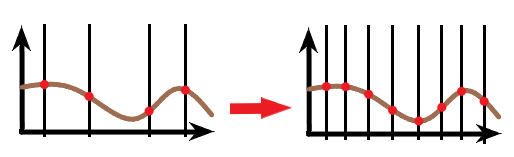
\includegraphics[height=6cm,width=1\textwidth,keepaspectratio]{f1.png}
        \caption{При увеличении количества ног увеличивается детализация картографируемой поверхности}
        \label{fig:f1.png}
    \end{subfigure}

    \begin{subfigure}{0.9\textwidth}
        \centering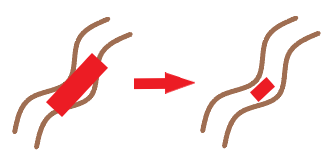
\includegraphics[height=6cm,width=1\textwidth,keepaspectratio]{f2.png}
        \caption{При увеличении количества ног, корпус робота увеличивается и он не может пройти часть препятствий}
        \label{fig:f2.png}
    \end{subfigure}

    \begin{subfigure}{0.9\textwidth}
        \centering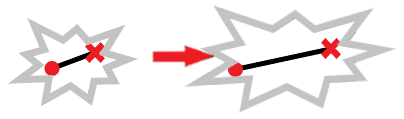
\includegraphics[height=6cm,width=1\textwidth,keepaspectratio]{f3.png}
        \caption{При изменении количества ног меняется проходимость системы}
        \label{fig:f3.png}
    \end{subfigure}

\caption{Критерии оптимизации конструкции робота}
\label{fig:opti_criteria}
\end{figure}
Изучая данные требования возможно заметить, что часть из них коррелируют друг с другом, а часть - диссонируют. Чем больше количество полученных точек на пройденной поверхности, тем выше будет детализация карты. Одним из способов увеличения детализации это увеличение количества ног у робота \pic{fig:f1.png}. С другой стороны, это увеличивает длину робота, а следовательно робот хуже сможет проходить узкие участки с обилием поворотов \pic{fig:f2.png}. Чем большее расстояние робот сможет пройти за одно и то же время, тем быстрее будет построена карта и робот меньше повлияет на окружающую среду при прочих равных условиях \pic{fig:f3.png}. 

Как итог возникает задача, которая не имеет одного лучшего решения. Следовательно, это мультикритериальная задача оптимизации.


Было решено, что цикловой движитель с одной степенью свободы в ноге лучше всего подходит для решения подобных задач.

Для цикловых движителей с одной степенью свободы в ноге вопрос о количестве ног не имеет однозначного решения. Поэтому необходимо провести структурный синтез, чтобы определить их количество. Данная задача решалась с помощью генетического алгоритма.

Генетический алгоритм это эвристический алгоритм поиска, используемый для решения задач оптимизации и моделирования путём случайного подбора, комбинирования и вариации искомых параметров с использованием механизмов, аналогичных естественному отбору в природе. Для решения задачи использовалась библиотека Deap и OpenAI.

Для создания подходящего робота, который может эффективно решать конкретные задачи, необходимо провести структурный синтез. Это означает, что оптимизируются такие характеристики робота, как количество ног, угол между ногами и т.д., используя алгоритмы оптимизации.

При оптимизации очень важно выбрать подходящую функцию пригодности. Иногда эта функция может быть явно выражена через аналитическую формулу: например, выражение общего материального объема робота как функции его геометрических параметров. Однако, в других случаях желаемая мера эффективности не может быть вычислена в явном виде и может быть получена только с помощью физического эксперимента или соответствующего моделирования. В данном случае важно максимизировать ходовые качества робота на различных сложных участках, и основным используемым показателем будет проходимость по местности. Генерируется семейство роботов, изменяя выбранные параметры конструкции робота, такие как количество ног.

Понятие сложности поверхности субъективно. Поэтому хорошей практикой ей генерация семейства проходимых поверхностей. Затем оценивается пригодность робота для ходьбы с помощью физической симуляции, во время которой робот будет проходить по местности. Также были получены параметризации различных генеративных моделей местности, чтобы было возможно на более позднем этапе исследовать влияние не только типа местности, но и параметров местности и, следовательно, на лучшие конструкции в зависимости от конкретной местности.

Для того чтобы направлять процесс поиска в пространстве возможных значений параметров, решено использовать модифицированный эволюционный алгоритм, который создает последовательные поколения конструкций с помощью соответствующих генетических операторов, играющих роль мутаций и скрещивания. После нескольких инициализаций и поколений были получены многообещающие результаты и полезные идеи, которые позволили создать конструкции, значительно улучшающие производительность, для достижения конечной цели - многоножек, способных преодолевать сложные участки местности.

\subsection{Математическая модель робота}
Исследуется механическая система, состоящая из твёрдых тел \eqref{eq:newton_euler}, движение которых описывается дифференциальными уравнениями вида:

\begin{align}
    \label{eq:newton_euler}
    M \dot{\vec{u}} = \vec{g} \\
    M = \begin{bmatrix}
    M_1 & \cdots  & 0 \\
    \vdots  & \ddots  & \vdots  \\ 
    0 & \cdots   & M_n 
    \end{bmatrix},\ M_i = \begin{bmatrix}
    m_i E_{3\times 3} & 0 \\ 
    0 & I_i 
    \end{bmatrix} \\
    \vec{u}_i^{\ T} = \begin{bmatrix}
        \vec{v}_i^{\ T} & \vec{\omega}_i^{\ T}
    \end{bmatrix} \\ 
    \vec{g}^{\ T} = \begin{bmatrix}
        \cdots \  \vec{F}_i^{\ T}, & (\vec{\tau}_i - \vec{\omega}_i \times I_i \vec{\omega}_i)^T\  \cdots 
    \end{bmatrix}
\end{align}
где, $M_i$~---~матрицы, содержащие массово-инерционные характеристики; $m_i$~---~масса тела; $I_i$~---~тензор инерции; $\vec{u_i}$~---~вектор обобщённых скоростей; $E$~---~единичная матрица; $\vec{g}$~---~вектор обобщённых сил; $\vec{v_i}$~---~вектор линейной скорости; $\vec{\omega_i}$~---~вектор угловой скорости; $\vec{F_i}$, $\vec{\tau_i}$~---~силы и моменты сил взаимодействия.

Тела, входящие в систему соединены между собой цилиндрическими шарнирами, которые описываются следующими связями и динамическими ограничениями:
\begin{align}
    \label{eq:kin_constr}
    \phi(q_{j_1},\ u_{j_1},\ \cdots,\ q_{j_k},\ u_{j_k},\ t) \geqslant  0 \\
    \vec{q}_i^{\ T} = \begin{bmatrix}
        \vec{x}_i^{\ T} & \vec{Q}_i^{\ T}
    \end{bmatrix} \\
    \dot{\vec{q}_i} = \begin{bmatrix}
    E_{3\times3} & 0\\ 
    0 & G(\vec{q}_i) 
    \end{bmatrix}\vec{u}_i  
\end{align}

\begin{align}
    \label{eq:phys_constr}
    \vec{g}_i = \tau_i^T \vec{z}_{i-1} -k\vec{v}_i \dot{\vec{q}_i} 
\end{align}
где через $\phi$ обозначена функция связи; $t$~---~время; $q_{j}$~---~вектор обобщенных координат, включающий в себя координаты центра масс $\vec{x_i}$ и кватернион $\vec{Q_i}$, описывающий ориентацию тела в пространстве; через $G(\vec{q}_i)$ обозначена матрица, вид которой зависит от выбранной системы координат и способа задания ориентации тела; $k$~---~ коэффициент вязкого трения в шарнире.

Контакт ног робота с опорной поверхностью \pic{fig:contact_interaction.png} описывается на базе модели сухого трения и выражатеся следующими уравнениями:

\begin{figure}[H]
    \centering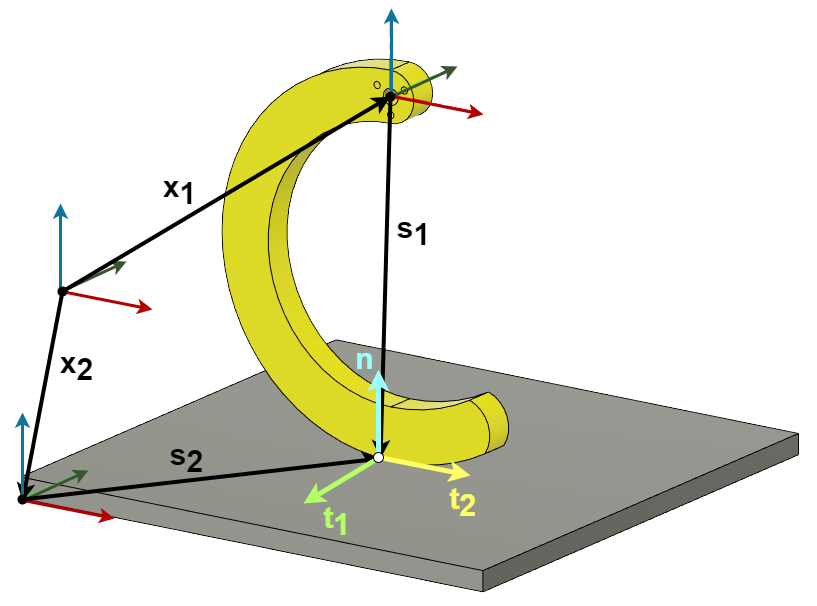
\includegraphics[height=9cm,width=1\textwidth,keepaspectratio]{images/contact_interaction.png}
    \caption{Описание переменных для модели взаимодействия опорной поверхности и ноги робота}
    \label{fig:contact_interaction.png}
\end{figure}

\begin{align}
    \label{eq:contact_inter}
    \phi_u(\vec{q}\ ) = g(\vec{q}\ ) \geqslant 0 \\ 
    g(\vec{q}\ ) = (\vec{x}_1 + \vec{s}_1 - \vec{x}_2 - \vec{s}_2) \cdot \vec{n} \\
    \frac{d }{d t}\phi_u(\vec{q}\ ) \approx \begin{bmatrix}
        \vec{n}^{\ T} & (\vec{s}_1 \times \vec{n})^T & -\vec{n}^{\ T} & (-\vec{s}_2 \times \vec{n})^T
    \end{bmatrix} \begin{bmatrix}
        \vec{v}_1\\ 
    \vec{\omega}_1\\ 
    \vec{v}_2\\
    \vec{\omega}_2\\
    \end{bmatrix}
\end{align} 

\begin{align}
    \label{eq:ground_inter}
\left\{\begin{matrix*}[l]
\mu f_n \geqslant \sqrt{f_1^2 + f_2^2}\\ 
\left\lVert \vec{v_t}\right\rVert (\mu f_n - \sqrt{f_1^2 + f_2^2}) = 0\\
\dfrac{\vec{f_t}}{\left\lVert \vec{f_t}\right\rVert } = - \dfrac{\vec{v_t}}{\left\lVert \vec{v_t}\right\rVert }
\end{matrix*}\right.
\end{align}
где, $\phi_u(\vec{q})$~---~функция связи; $ \mu $~---~ коэффициент трения между ногой и опорной поверхностью;  радиус-векторы $\vec{x}_{1,2},\ \vec{s}_{1,2}$ и орты координатных осей $\vec{t}_{1,2}, \vec{n}$ показаны на рисунке \pic{fig:contact_interaction.png}; $ f_{1,2} $~---~значения сил трения вдоль осей $t_{1,2}$ соответственно.

\subsection{Представление робота}

Геометрическая модель робота представлена в виде трехмерного параллелепипеда. Количество движителей по каждому из бортов обозначается через $\gamma$. Разность фаз между соседними движителями обозначается через  $\alpha$ \pic{fig:best_gen_robot.jpg}.

\begin{figure}[H]
    \centering
    \begin{tikzpicture}
        % Include the image in a node
        \node [above right, inner sep=0] (image) at (0,0)
        {\centering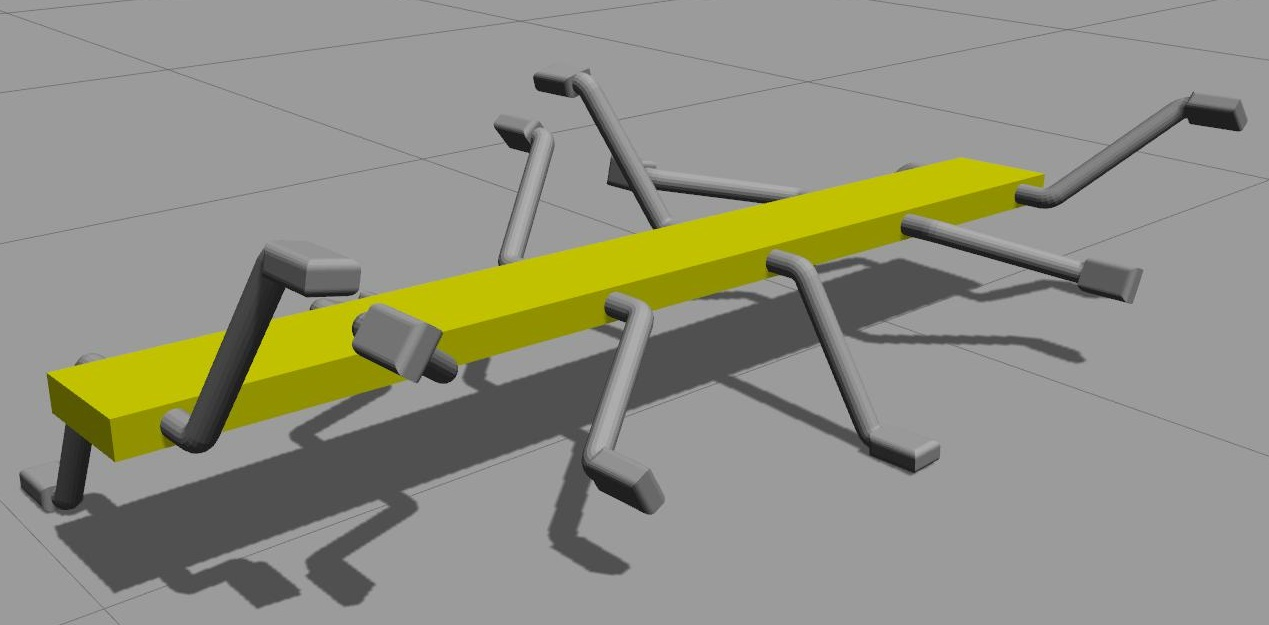
\includegraphics[height=10cm,width=0.8\textwidth,keepaspectratio]{best_gen_robot.jpg}};
        % Create scope with normalized axes
        \begin{scope}[
                x={($ 0.1*(image.south east)$)},
                y={($ 0.1*(image.north west)$)}]
            % Labels
            \draw [green, very thick,
                decorate,
                decoration = {brace,
                        raise=5pt,
                        amplitude=5pt,
                        aspect=0.5}] (1.4,3.6) --  (8.1,6.8)
            node[rounded corners=3pt, pos=0.5,above left =14pt,black,fill=white]{\tiny $(\gamma - 1) h_{\text{leg}}\sin(\alpha)$};

            \draw[stealth-, very thick,green] (9.5,7.8) -- (7.8,1.94);
            \draw[stealth-, very thick,green] (1.5,2.8) -- (7,1)
            node[rounded corners=3pt,right,black,fill=white]{\tiny $\gamma = 6$};

            \draw[thin,green] (6.7,4) -- (5.75,9);
            \draw[thin,green] (4.85,3.5) -- (5.75,9);
            \draw[thin,green,stealth-stealth] (6.32,6) arc (-79.2:-99.2:3) node [rounded corners=3pt,below = 2pt,black,fill=white, midway] {\tiny $\alpha$};
        \end{scope}
    \end{tikzpicture}
    \caption{Схема модели робота для генетического алгоритма}
    \label{fig:best_gen_robot.jpg}
\end{figure}

Эту задачу можно сформулировать как мультикритериальную задачу оптимизации, где необходимо максимизировать дистанцию, пройденную за фиксированное время, и минимизировать длину робота \eqref{eq:second}. Параметрами индивида являлись $\gamma$ и $\alpha$.

\begin{align}
    \label{eq:second}
    F \rightarrow max = \beta \left( {\omega}_{1} \cdot \overbrace{\delta}^{\text{Distance}} + {\omega}_{2} \cdot \overbrace{\frac{1}{(\gamma - 1) h_{\text{leg}}\sin(\alpha)}}^{\text{Simplified body length}}\right) + \\ \nonumber + (1 - \beta) {\delta}^{{\omega}_{1}} {\left( \frac{1}{(\gamma - 1)h_{\text{leg}}\sin(\alpha)}\right)}^{{\omega}_{2}}
\end{align}
где \nom{$\delta$}{пройденная дистанция}, \nom{$\beta$}{адаптивный параметр}, \nom{${\omega}_{1,2} \in  [ 0..1 ] $}{весовые коэффициенты}.


Модель робота должна быть реализована в формате URDF. Это язык разметки формата XML для представления модели робота. Но это старый формат, и когда модель импортируется в Gazebo, URDF преобразуется в формат SDF. Это важно, потому что некоторые функции не реализованы в чистом URDF. В нашем случае это шарнир коробки передач. Но можно вставить код в формат SDF, и он будет работать правильно.

\subsection{Генерирование местности, по которой будет проходить робот}
Прежде чем говорить о генерировании местности, необходимо обосновать данное решение. Глобальная задача это оценить сложность рельефа. Основными найденными подходами к оценке рельефа являются.
\begin{enumerate} 
    \item Анализ множества физических свойств поверхностей, таких как ковер или линолеум, с точки зрения максимальной скорости, мощности и других параметров робота при их прохождении \cite{Altendorfer2001}.
    \item Построение конкретной местности, которая является достаточно сложной в субъективном плане. В задании Rough Terrain Task в DARPA's Virtual Robotics Challenge используется этот подход. Таким образом тестировался робот ATLAS \cite{feng_Optimizationbased_2015} \pic{fig:terrain_assesment/c2_paper.jpg}.
          
          \begin{figure}[H]
              \centering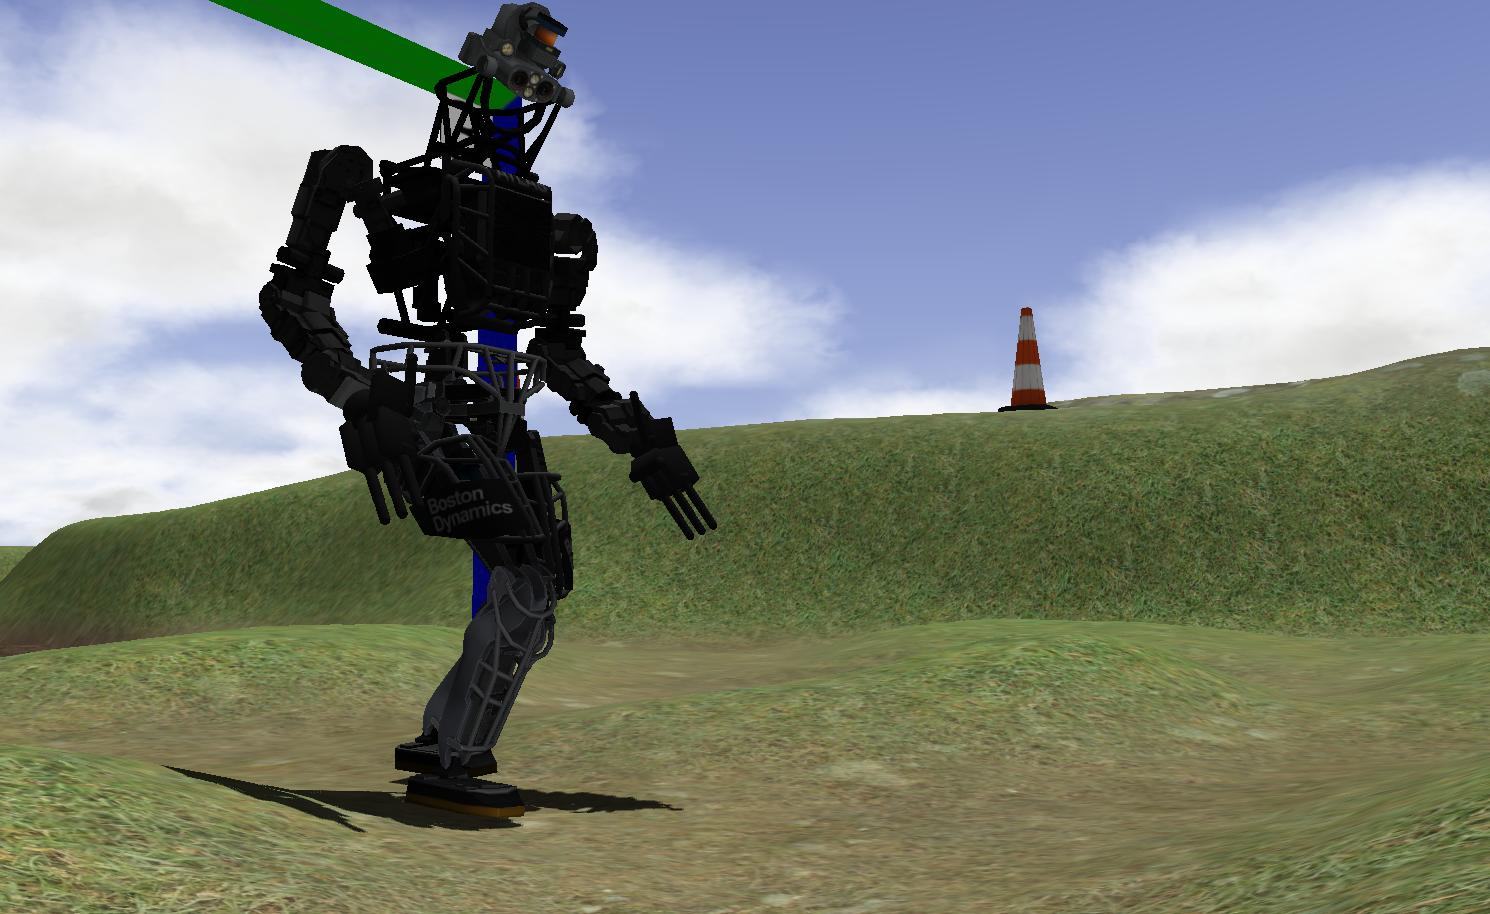
\includegraphics[height=6cm,width=1\textwidth,keepaspectratio]{terrain_assesment/c2_paper.jpg}
              \caption{Задание на пересеченной местности в конкурсе виртуальной робототехники DARPA}
              \label{fig:terrain_assesment/c2_paper.jpg}
          \end{figure}
          
    \item Оценка местности в соответствии с возможностями робота. Она основывается на максимальном перепаде высот, который может преодолеть робот. Если робот не может его преодолеть, значит, местность неудовлетворительная \cite{hung_Advanced_2004,Howard2000} \pic{fig:terrain_assesment/c3_paper.png}.
          
          \begin{figure}[H]
              \centering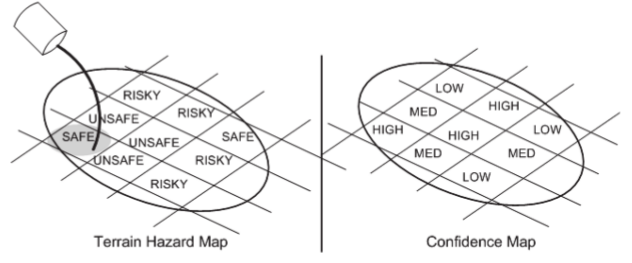
\includegraphics[height=6cm,width=1\textwidth,keepaspectratio]{terrain_assesment/c3_paper.png}
              \caption{Пример карт местности: карта опасности местности и карта достоверности местности}
              \label{fig:terrain_assesment/c3_paper.png}
          \end{figure}

    \item Оценка по карте с использованием ряда анализируемых параметров, таких как дисперсия, дальность, тип почвенно-растительного покрова, количество треугольных граней и так далее \cite{hung_Advanced_2004}.
    \item Получение искусственных поверхностей на основе параметров генерации. Первая версия этой идеи была связана с получением жестких ландшафтов с квадратной сеткой, где каждая ячейка имеет некоторую высоту \cite{sancho-pradel_Survey_2010} \pic{fig:terrain_assesment/c1_paper.png}.
          
          \begin{figure}[H]
              \centering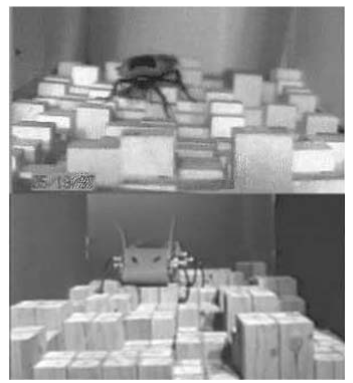
\includegraphics[height=8cm,width=1\textwidth,keepaspectratio]{terrain_assesment/c1_paper.png}
              \caption{Рельеф с параметризованными ячейками}
              \label{fig:terrain_assesment/c1_paper.png}
          \end{figure}
\end{enumerate}

После тщательного рассмотрения было решено, что последний подход с некоторыми модификациями и расширениями лучше всего подходит для нашей задачи.

Параметры местности, которые могут быть изменены, следующие:
\begin{itemize}
\item номер ширины и длины клетки;
\item диапазон высоты клетки начало и конец;
\item ширина и длина клетки;
\item 2(3) измерения местности (рис.~\ref{fig:terrain_1});
\item параметр распределения (рис.~\ref{fig:terrain_2}).
\end{itemize}

Для выбора высоты клеток были проведены эксперименты.
Существует 3 диапазона, определяющих свойства местности, которые изображены ниже (рис.~\ref{fig:range}).

\begin{figure}[H]
\centering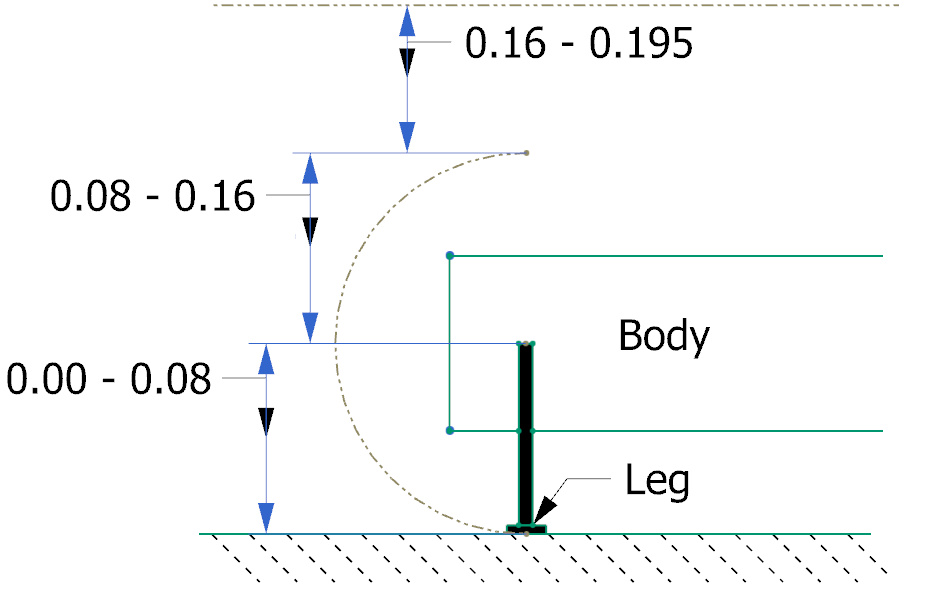
\includegraphics[width=0.5\textwidth]{from_master/ranges}\\
\caption{Три диапазона для оценки рельефа местности}
\label{fig:range}
\end{figure}

Для каждого диапазона было сгенерировано 20 местностей и 50 роботов. Каждый робот пытается пройти все местности. У робота есть 4 секунды на попытку. Успешные попытки засчитывались. Результаты можно увидеть в таблице \ref{tabular:ranges}.

\begin{table}[H]
\caption{Процентное соотношение между диапазонами и успешными попытками}
\label{tabular:ranges}
\centering
\begin{tabular}{c|c}
 \textbf{Диапазон} & \textbf{Процент успешных попыток}\\
 \hline
0.00 -- 0.08 & 99.7 \\ 
0.08 -- 0.16 & 79.7 \\
0.16 -- 0.195 & 47.3 \\
\end{tabular}
\end{table}


Таким образом, было решено, что второй и первый диапазоны (0.00 - 0.16) будут использоваться в алгоритме оптимизации.

В информатике генетические алгоритмы - это адаптивные эвристические алгоритмы поиска, основанные на эволюционных концепциях. Они представляют собой интеллектуальную параллельную эксплуатацию пространства проектирования и могут быть использованы для решения проблем оптимизации, не обязательно оптимизируя, но часто получая близкие к оптимальным решения. 

Реализация генетического алгоритма основана на библиотеках Deap  и OpenAI-ES \cite{DEAP_JMLR2012,salimans_Evolution_2017}.

Генетический код особи содержит 3 основных гена: количество ног, угол между двумя соседними ногами и волновое смещение между сторонами, а также 1 дополнительный ген~--- пройденная дистанция, который зависит от других генов и поэтому не участвует в процедурах скрещивания и мутации. 

Алгоритм заключается в следующем. После случайной генерации начальной популяции, популяция эволюционирует с помощью трех операторов: селекции, основанного на повышенной вероятности выживания сильнейшего; скрещивания, который представляет собой спаривание между особями и мутации, которая вносит случайные изменения в значения генов отдельных особей.

Процедура селекции, реализующая турнирный подход, была взята из библиотеки Deap без изменений. 

Были написаны собственные реализации скрещивания и мутации:
\begin{enumerate}
\item Для скрещивания используется общая функция с некоторыми дополнениями. Каждая особь имеет 4 гена, но четвертый ген (расстояние) зависит от других генов. Поэтому функция скрещивания должна работать только с первыми тремя характеристиками.

\item Мутация: Аналогично скрещиванию, используется только 3 поля. Модель робота имеет ограничения, например по максимальной длине, поэтому с некоторой заданной вероятностью каждая из характеристик может быть изменена в определенном интервале. Допускается осуществление с одной и той же особью нескольких мутаций, но с каждым разом вероятность мутации уменьшается. 
\end{enumerate}

Этот псевдокод дает высокоуровневое описание всего алгоритма.

\begin{algorithm}[H]
\caption{Верхеуровневый генетический алгоритм\label{high_level}}
% \begin{small}
\KwIn{$\alpha$ -- количество поколений, $\beta$ -- количество индивидов, $\gamma$ -- количество территорий}
\KwOut{Хорошие параметры для робота}
\Begin{
Генерация семейства поверхностей\;
случайная генерация первого поколения индивидов\;
\For{$i = 0$ \KwTo $\alpha$}{
\For{$j = 0$ \KwTo $\beta$}{
$distance = 0$\;
\For{$k = 0$ \KwTo $\gamma$}{
Начало симуляции\;
$distance += cur\_distance$\;
}
$avg\_distance = distance / \gamma$\;
высчитывание фитнес функции\;
}
выбор лучших родителей\;
скрещивание выбранных родителей\;
мутация генов\;
}
}
% \end{small}
\end{algorithm}

Было проведено два эксперимента. В первом эксперименте искались лучшие параметры робота для территории T1. Во втором эксперименте рассматривалась зависимость от разных типов ландшафтов при меньшем количестве индвидов. Весовые коэффициенты $\omega_1,\ \omega_2$ варьировались, но здесь и далее приведены данные, полученные при $\omega_1 = 0.6,\ \omega_2 = 0.4$. 

\begin{figure}[H]
    \begin{subfigure}{0.33\textwidth}
    \centering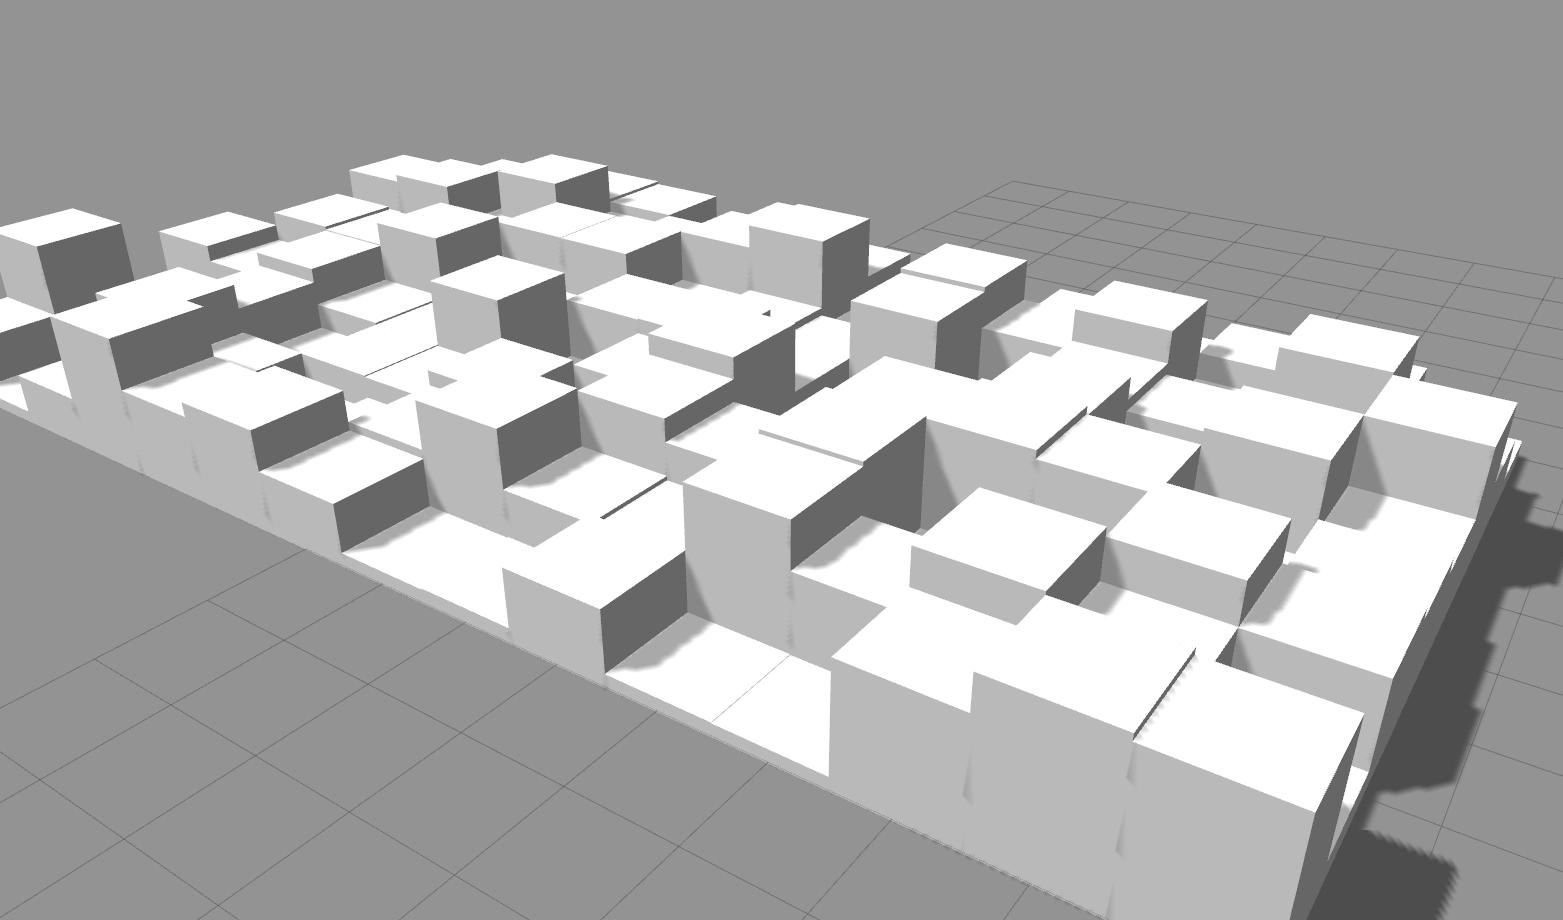
\includegraphics[width=0.8\textwidth]{terrain_1} 
    \caption{T1: 3D-боксы с равномерным распределением высоты}
    \label{fig:terrain_1}
    \end{subfigure}
    \begin{subfigure}{0.33\textwidth}
    \centering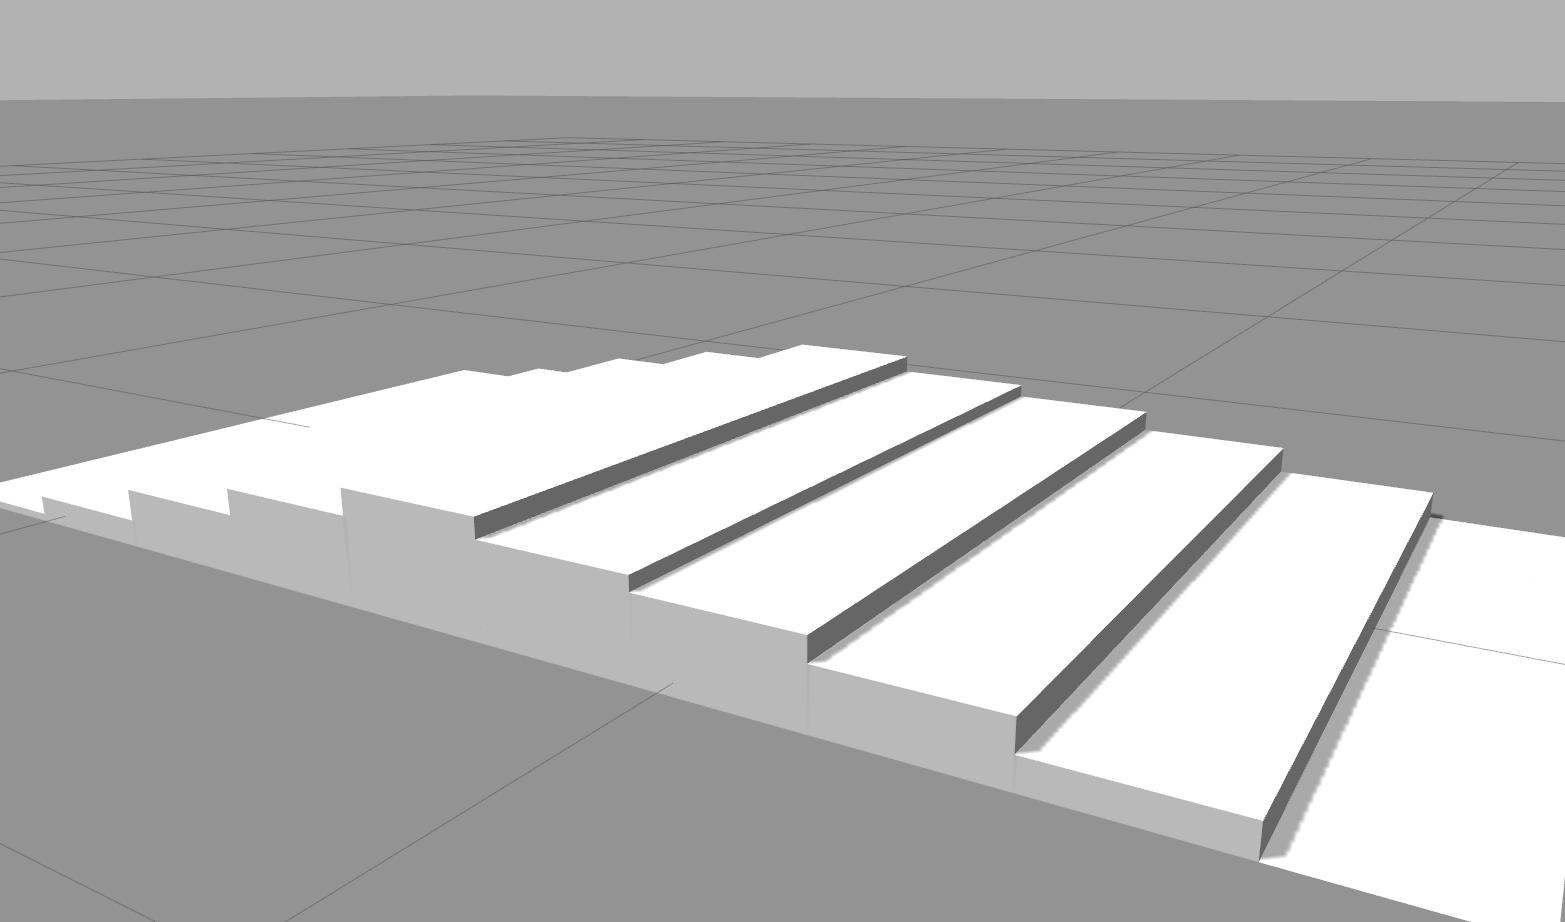
\includegraphics[width=0.8\textwidth]{terrain_2} 
    \caption{T2: 2D-полосы с гауссовой функциональной высотой}
    \label{fig:terrain_2}
    \end{subfigure}
    \begin{subfigure}{0.33\textwidth}
    \centering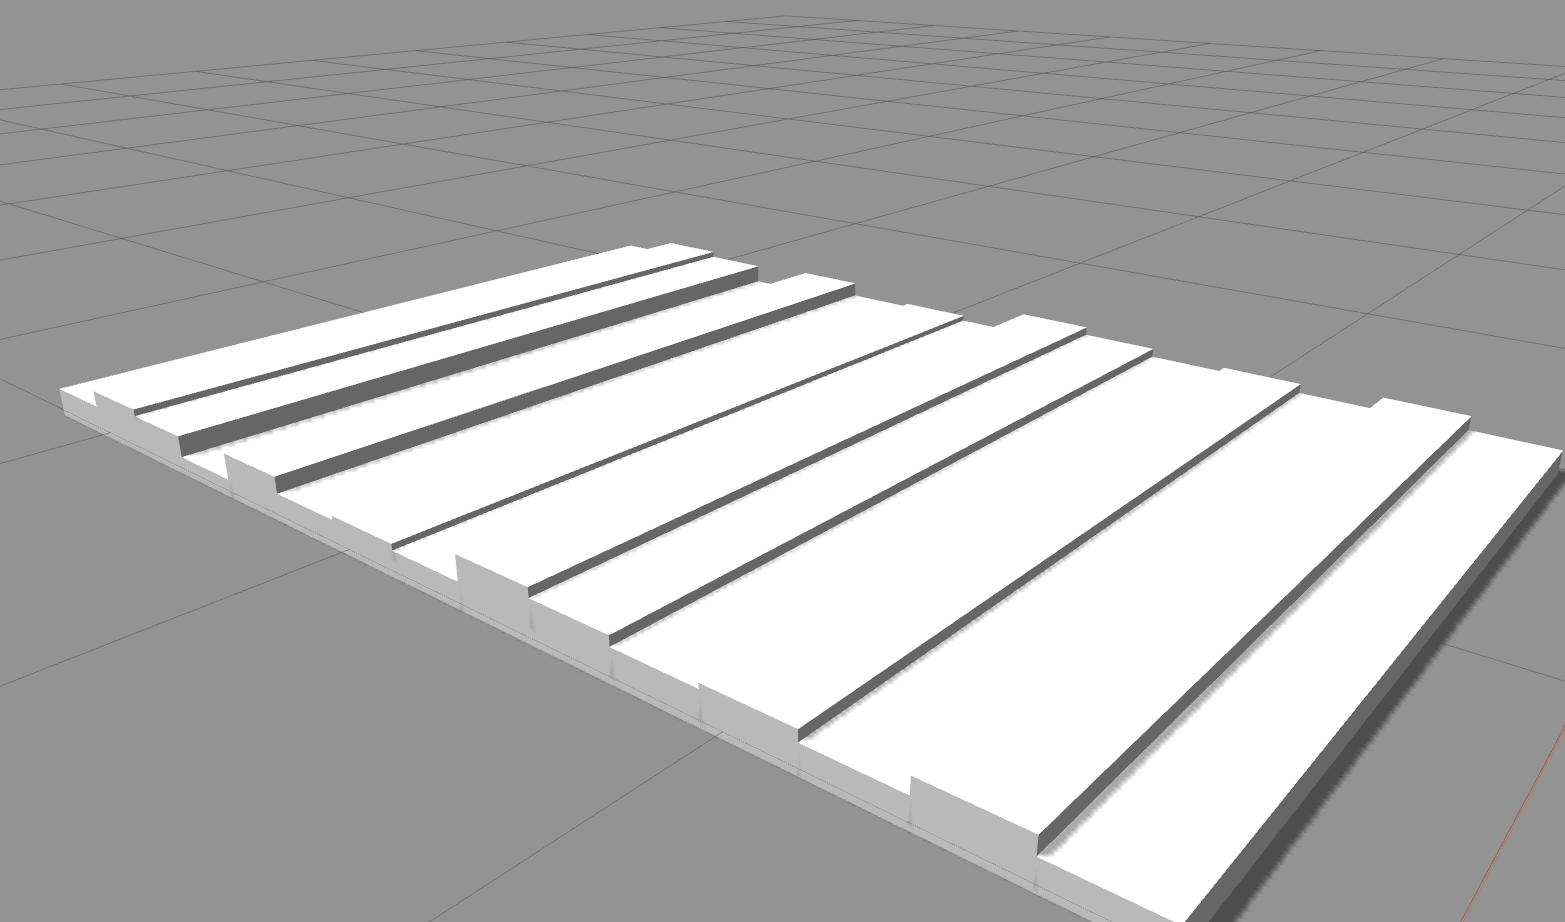
\includegraphics[width=0.8\textwidth]{terrain_3}
    \caption{T3: 2D-полосы с распределением высоты по гауссовской функции)}
    \label{fig:terrain_3}
    \end{subfigure}
     
    \caption{Примеры сгенерированных территорий}
    \label{fig:terrains}
\end{figure}

\begin{figure}[H]
    \centering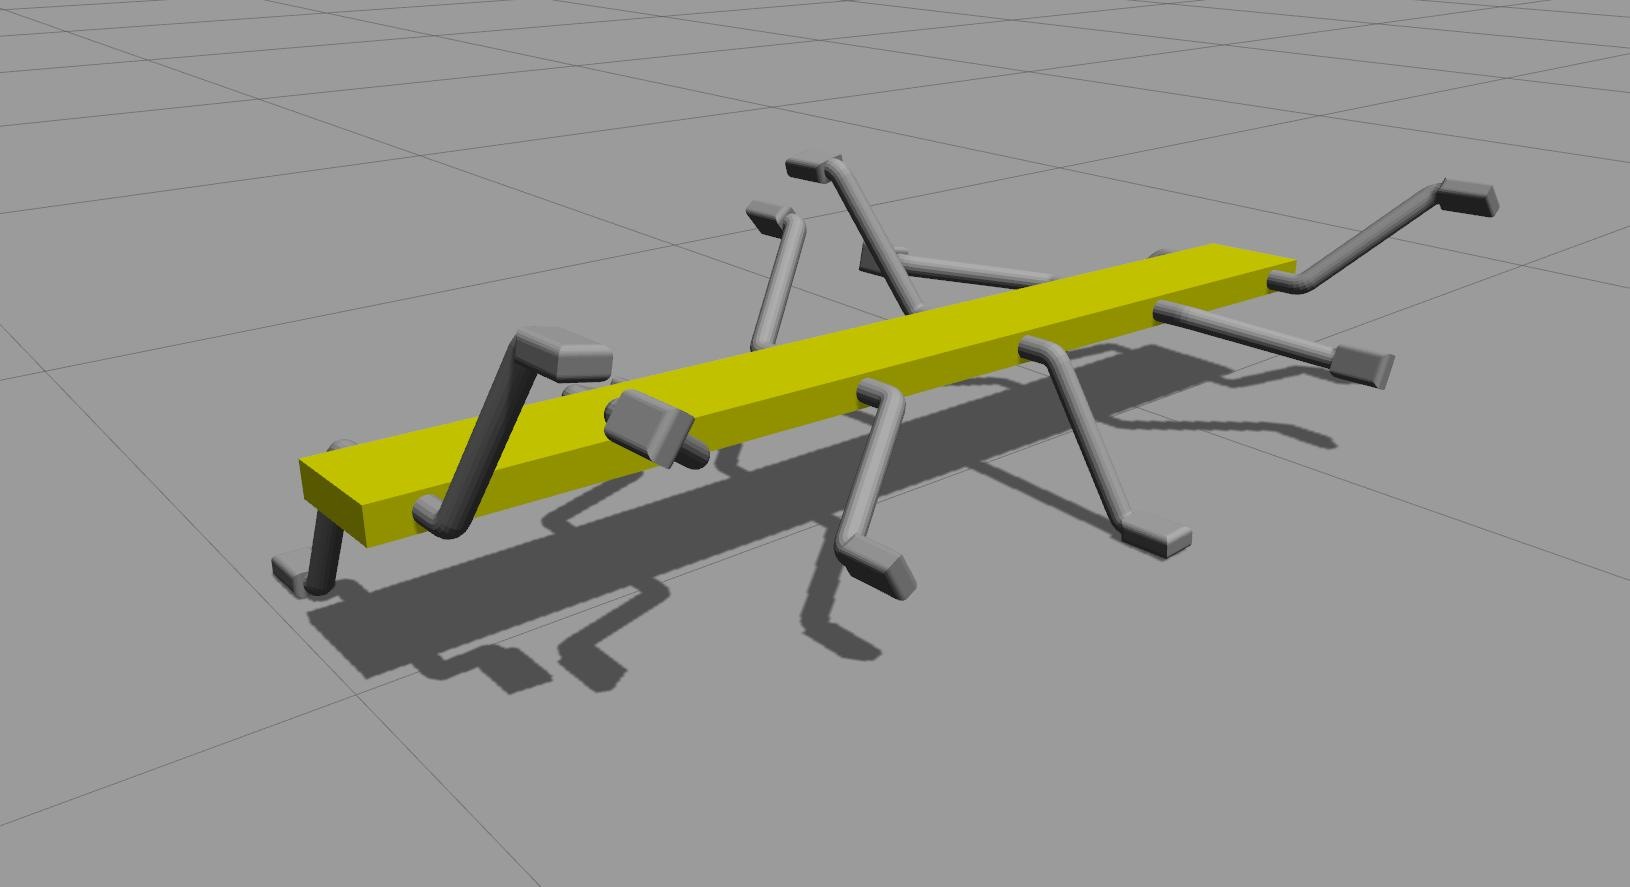
\includegraphics[width=0.6\textwidth]{from_master/best_robot}\\
    \caption{Робот с результирующими результатами}
    \label{fig:best_robot}
    \end{figure}
    \begin{figure}[H]
    \centering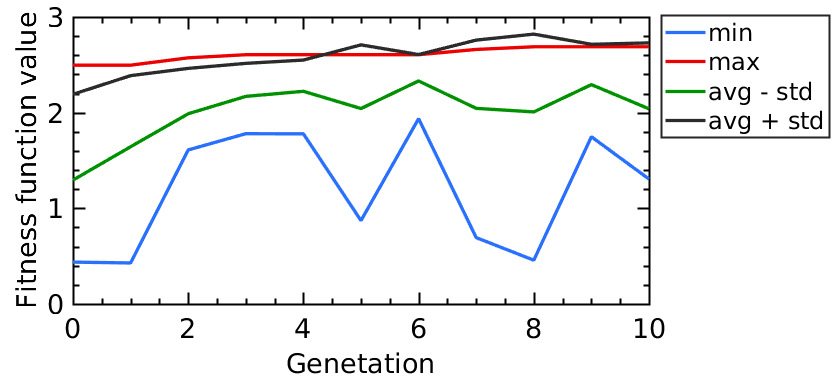
\includegraphics[width=0.6\textwidth]{from_master/best_robot_200_plot}\\
    \caption{Среднее значение фитнес-функции $\pm$ std на поколение
    Минимальное и максимальное значения фитнес-функции на поколение}
    \label{fig:plot4}
    \end{figure}
    
    Весовые коэффициенты настраивались в зависимости от выбора приоритета. Невзирая на выбранные коэффициенты, оптимальным набор ног начинался с 8 и заканчивался 14. Это объясняется критерием статического равновесия, который, как оказалось, увеличивает проходимость механизма. В данном случае 4 ноги всегда будут касаться пола. 
    
    Первый эксперимент: каждый робот проходил 10 разных ландшафтов по 9 секунд каждую. Второй эксперимент: она имеет те же параметры, что и первая фаза, но с измененным размером популяции. 
    
    В соответствии с таблицей \ref{tabular:Table2} (весовые коэффициенты равны 0.6 и 0.4 соответственно) видна сходимость в параметрах. Видео прохождения препятствия лучшим индивидом \quad
    \qrcode[height=1.5cm]{https://youtu.be/DcovvkTZgsg}


\begin{table}[ht]
\centering
\caption{Зависимость между статистикой целевой функции и типами поверхности}
\label{tabular:Table2}
\begin{tabular}{c|c|c|c}
    \rowcolor{Gray}
\textbf{Территория, популяция} & \textbf{Параметры} & \textbf{AVG} & \textbf{STD}\\
\hline
\textbf{T1 \pic{fig:terrain_1}, 110} & (6, 72) & 2.38 & 0.34
\\
\rowcolor{LightGray}
\textbf{T2 \pic{fig:terrain_2}, 55}& (5, 68) & 1.95 & 0.35
\\
\textbf{T3 \pic{fig:terrain_3}, 55} & (6, 77) &  2.08 & 0.33 \\
\hline
\end{tabular}
\end{table}

Одним из основных результатов исследования, полученных при варьировании значений весовых коэффициентов $\omega$ является зависимость между количеством ног и пройденной дистанцией \pic{fig:box_plot_structural_synthesis.png}, которая показала наличие локального оптимума при количестве ног у робота в диапазоне от 8 до 14. 

\begin{figure}[H]
    \centering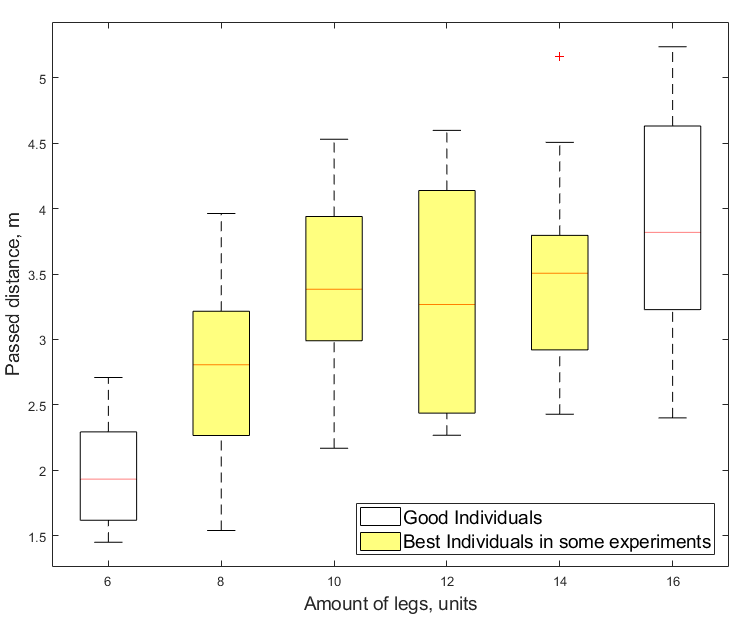
\includegraphics[height=10cm,width=1\textwidth,keepaspectratio]{images/box_plot_structural_synthesis.png}
    \caption{Зависимость между количеством ног и пройденной дистанцией}
    \label{fig:box_plot_structural_synthesis.png}
\end{figure}

Автор полагает, что этот факт может быть объяснён следующими соображениями. С одной стороны, слишком много ног значительно удлиняет корпус робота, что снижает его профильную проходимость за счёт того, что робот с большей вероятностью может задеть выступы при движении. С другой стороны при слишком малом количестве ног происходит потеря статической устойчивости робота. Поскольку для гарантированного обеспечения статической устойчивости необходимо обеспечить контакт не менее, чем 4 ног с опорной поверхностью в каждый момент времени, то естественным ограничением является 8 ног у робота.


\section{Задача оптимизации колебаний робота при походке}
Несмотря на то, что каждая нога робота может двигаться независимо, что позволяет получать абсолютно разные походки, возможно определить оптимальный угол между ногами робота при движении по плоскости. Под оптимальностью подразумевается максимальный клиренс и минимальные колебания системы. Клиренс это расстояние от корпуса робота, до опорной поверхности. Это позволит быстро преодолевать прямые участки с минимальным риском для оборудования, находящегося в роботе.

Задача целевой функции --- максимизировать положение $Z$ и минимизировать $STD$. Одновременно необходимо сделать минимальным $RMS$ и $STD$ углов в обоих направлениях (крен и тангаж). Важным моментом является и направление движения.

Целевая функция имеет следующий вид:
\begin{align}
    \label{eq:objective}
    F = \sum\limits_{i=1}^4 \omega_{i} \cdot (\frac{1}{\omega_{z1}Z_{rms}^i - \omega_{z2}Z_{std}^i}  + ( \omega_{p1}\alpha_{rms}^i + \omega_{p2}\alpha_{std}^i) + \nonumber \\\ + (\omega_{r1}\beta_{rms}^i + \omega_{r2}\beta_{std}^i)) \rightarrow min
\end{align}
где надпись \nom{$i =\{1,2,3,4\}$}{среднее значение a, которое принимается из 1 - движение вперед, 2 - движение влево, 3 - движение вправо, 4 - вращение}; \nom{$Z$}{положение по оси Z}; \nom{$\alpha, \beta$}{значения ориентации по крену и шагу}; \nom{$\omega_{i}$}{весовой коэффициент для каждого направления}, \nom{${\omega}_{z,roll,pitch}$}{весовые коэффициенты}.

Возможно решить задачу полным перебором, так как надо проверить 36 углов ~$\cdot$ 4 направления ~$\cdot$ 100 экспериментов для каждого направления ~$\cdot$ 144 шага в каждом.

Есть пример, который описывает два возможных движения: вперед и скольжение. Результаты о положении почти одинаковы для обоих типов.

\begin{figure}[H]
\begin{subfigure}{1\textwidth}
\centering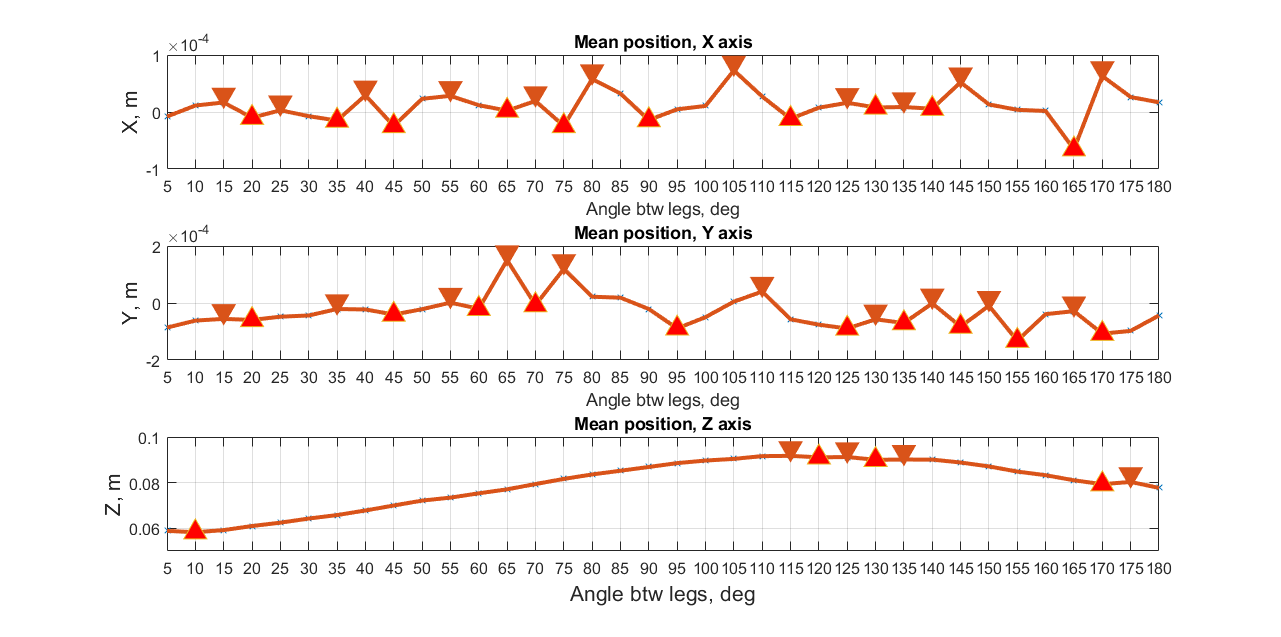
\includegraphics[width=0.9\textwidth]{from_master/forwardBestMean} 
\caption{Среднее значение из данных о положении для обоих типов движения}
\label{fig:forwardBestMean}
\end{subfigure}

\begin{subfigure}{1\textwidth}
\centering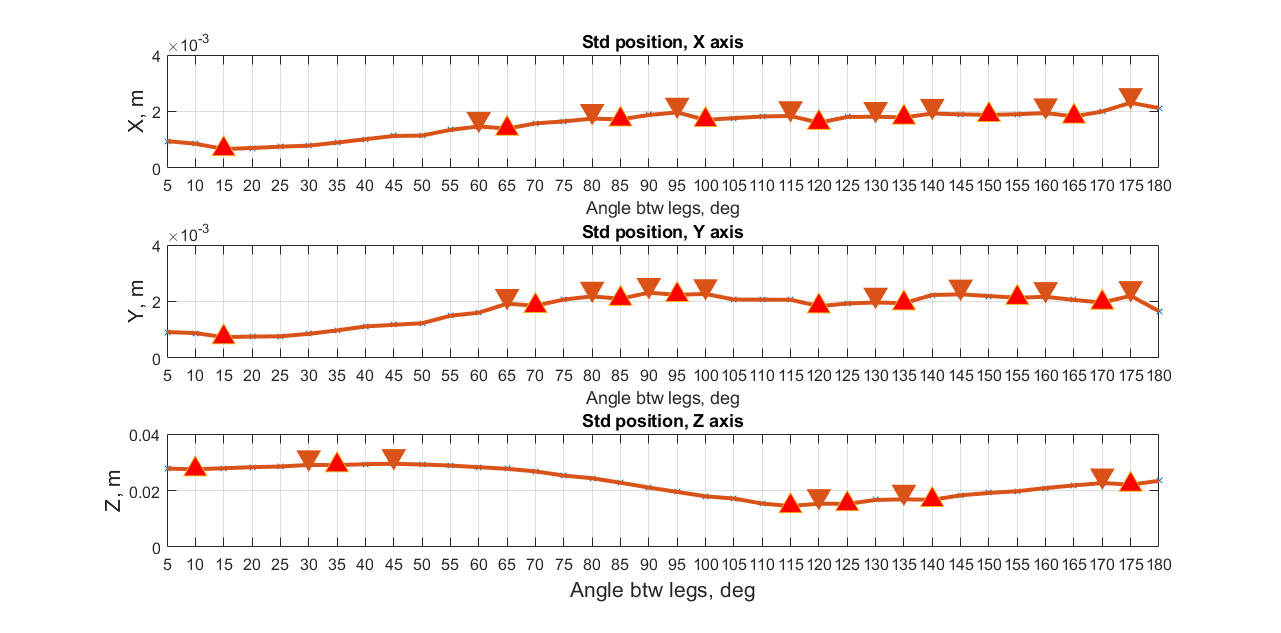
\includegraphics[width=0.9\textwidth]{from_master/forwardBestSTD} 
\caption{STD из данных о положении для обоих типов движения}
\label{fig:forwardBestSTD}
\end{subfigure}
 
\caption{Данные о положении для обоих типов движения}
\label{fig:forwardPosion}
\end{figure}

\begin{figure}[H]
\centering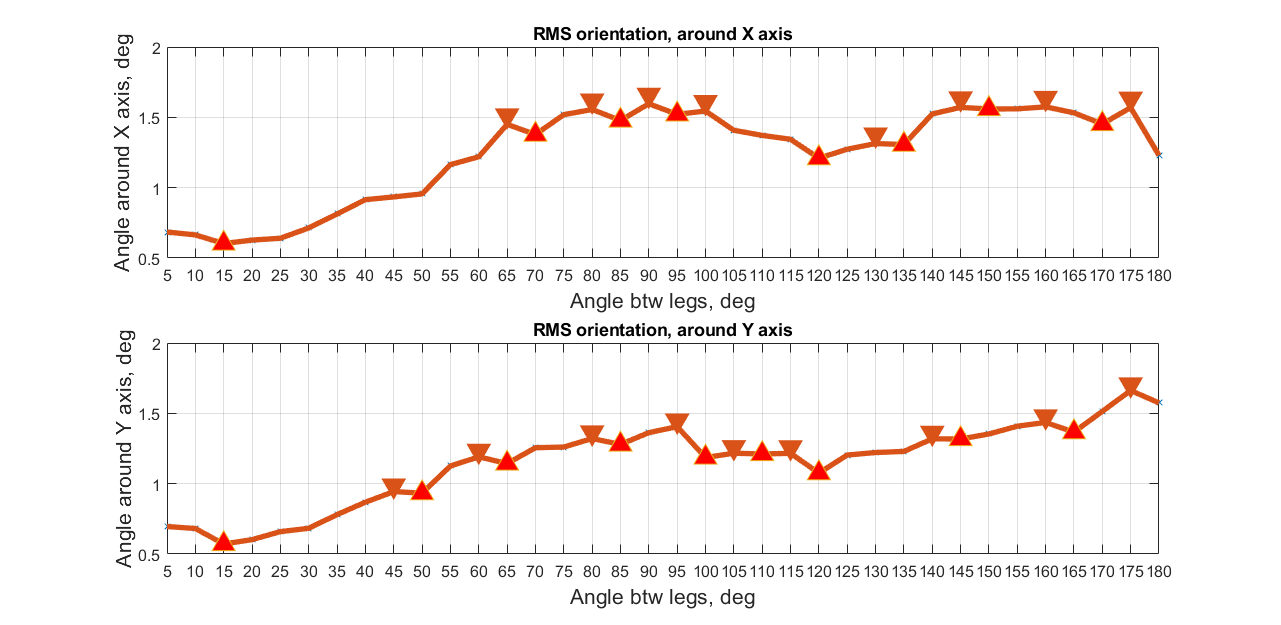
\includegraphics[width=0.9\textwidth]{from_master/forwardBestRMSrot} 
\caption{RMS из данных об ориентации для типа движения вперед}
\label{fig:forwardBestRMSrot}
\end{figure}

\begin{figure}[H]
\centering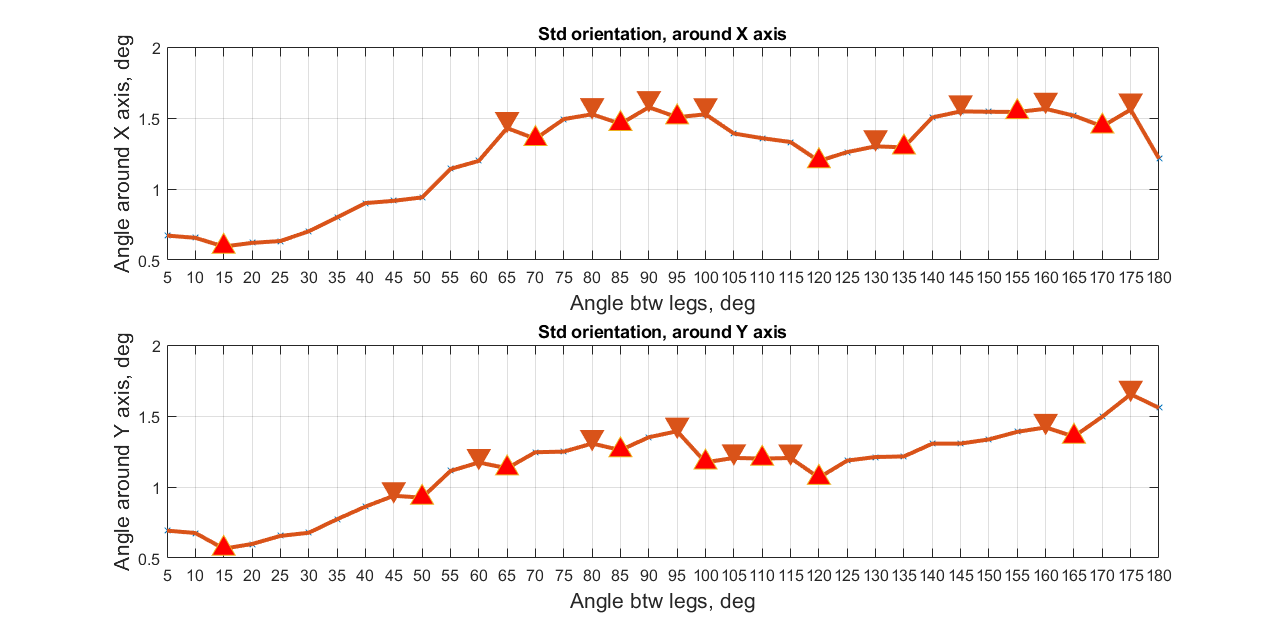
\includegraphics[width=0.9\textwidth]{from_master/forwardBestSTDRot} 
\caption{STD из данных об ориентации для типа движения вперед}
\label{fig:forwardBestSTDRot}
\end{figure}

\begin{figure}[H]
\begin{subfigure}{1\textwidth}
\centering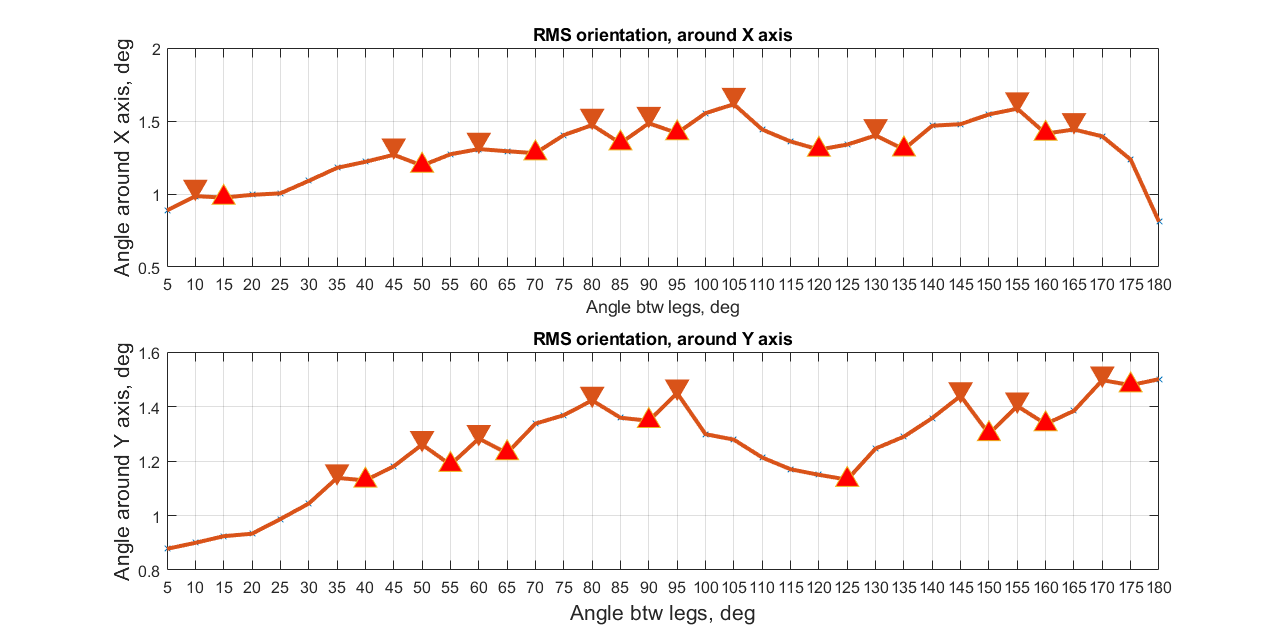
\includegraphics[width=0.9\textwidth]{from_master/slideBestRMSrot} 
\caption{RMS из данных об ориентации для типа движения вбок}
\label{fig:slideBestRMSrot}
\end{subfigure}

\begin{subfigure}{1\textwidth}
\centering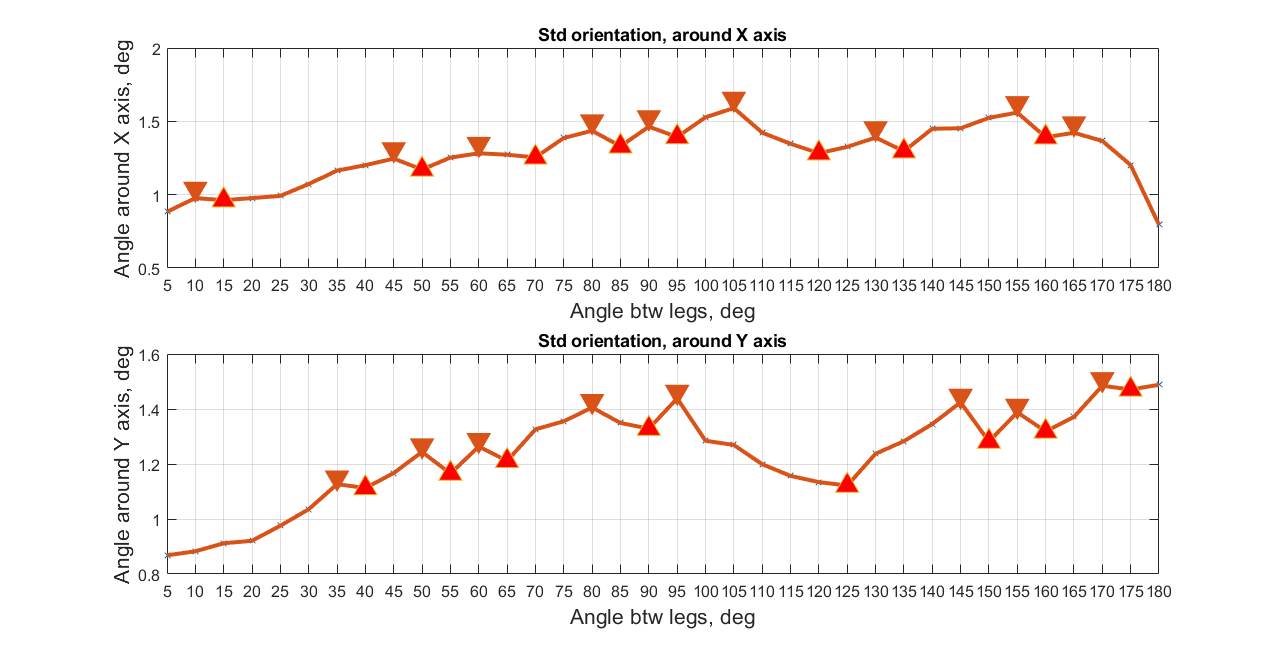
\includegraphics[width=0.9\textwidth]{from_master/slideBestSTDRot} 
\caption{STD из данных об ориентации для типа движения вбок}
\label{fig:slideBestSTDRot}
\end{subfigure}
 
\caption{из данных об ориентации для типа движения вбок}
\label{fig:slideOrientation}
\end{figure}

В результате работы получен угол между ногами равный 120 градусам. Это можно объяснить, потому что это периодическая функция, а обычно этот тип функций дает подходящие результаты.

\section{Оптимизация конструкции робота для прохождения узких участков}

В первом пункте требований к движителю (начало главы) стоит требование, чтобы робот не застревал при поворотах. Проблема застревания решается с помощью изменения угла между ногой и корпусом робота.

Возможность двигаться во все направления без смены ориентации сильно повышает проходимость робототехнической системы во многих случаях. Классическая компоновка многоногого шагающего робота с одной степенью свободы в ноге не позволяет перемещаться таким образом. Но если воспользоваться концептом, который используется в всенаправленных колесах, то шагающий робот с одной степенью свободы в ноге сможет перемещаться всенаправленно без смены ориентации.

\begin{figure}[H]
    \centering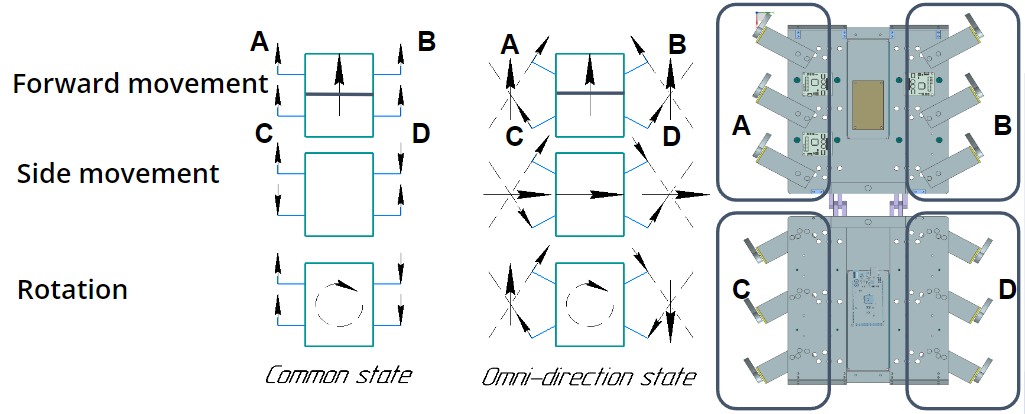
\includegraphics[height=10cm,width=1\textwidth,keepaspectratio]{omni_rot.png}
    \caption{Векторное представление сил в классическом и всенаправленном состоянии}
    \label{fig:omnidirection}
\end{figure}

На рисунке \ref{fig:omnidirection} представлена иллюстрация данной концепции: для того, чтобы робот двигался во всех направлениях, необходимо разбить ноги на группы, чтобы получилось 4 группы A-D.

Если сравнивать с классической компоновкой роботов (угол между корпусом робота и осью вала привода ноги равен 90 градусов), то вектор внешних сил будет таким, как на левой части рис. \ref{fig:omnidirection}. Стрелка в центре робота — суперпозиция всех сил. Если изменить угол оси привода ноги в соответствии с предлагаемой концепцией, то возможно получить значения суперпозиции сил, представленные на рис. \ref{fig:omnidirection} в центре. То есть, чтобы переместить корпус робота направо, группы А и D должны вращать ноги в одну сторону, а группы C и B — в противоположную. Правая часть рисунка иллюстрирует расположение групп ног на исследуемом роботе. 

\section{Разработанные концепции робота}

В рамках исследования было разработано четыре концепции робота СтриРус. В таблице \ref{tabular:robot_comparison_body} в строке недостатки объясняются основные причины перехода из одной итерации к другой. Концептуально было замечено, что высота ноги и наличие сегмента разительно влияет на проходимость конструкции. \quad \qrcode[height=1.5cm]{https://youtu.be/EQ6oGZVDpoc}

\begin{figure}[H]
    \centerfloat{
        \hfill
        \subcaptionbox[List-of-Figures entry]{Первая итерация\label{fig:strirus_0}}{%
            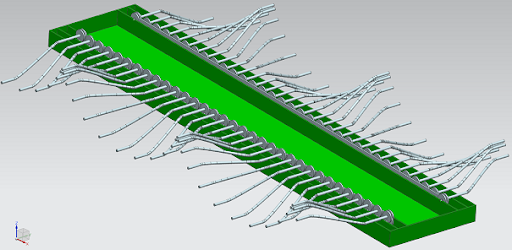
\includegraphics[width=0.49\linewidth]{strirus_0.png}}
        \hfill
        \subcaptionbox[List-of-Figures entry]{Вторая итерация \label{fig:strirus_1}}{%
            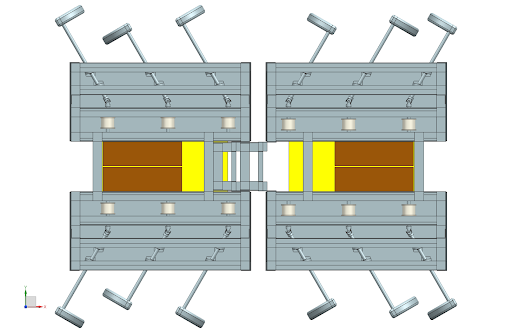
\includegraphics[width=0.49\linewidth]{strirus_1.png}}

        \hfill
        \subcaptionbox{Третья итерация\label{fig:strirus_2}}{%
        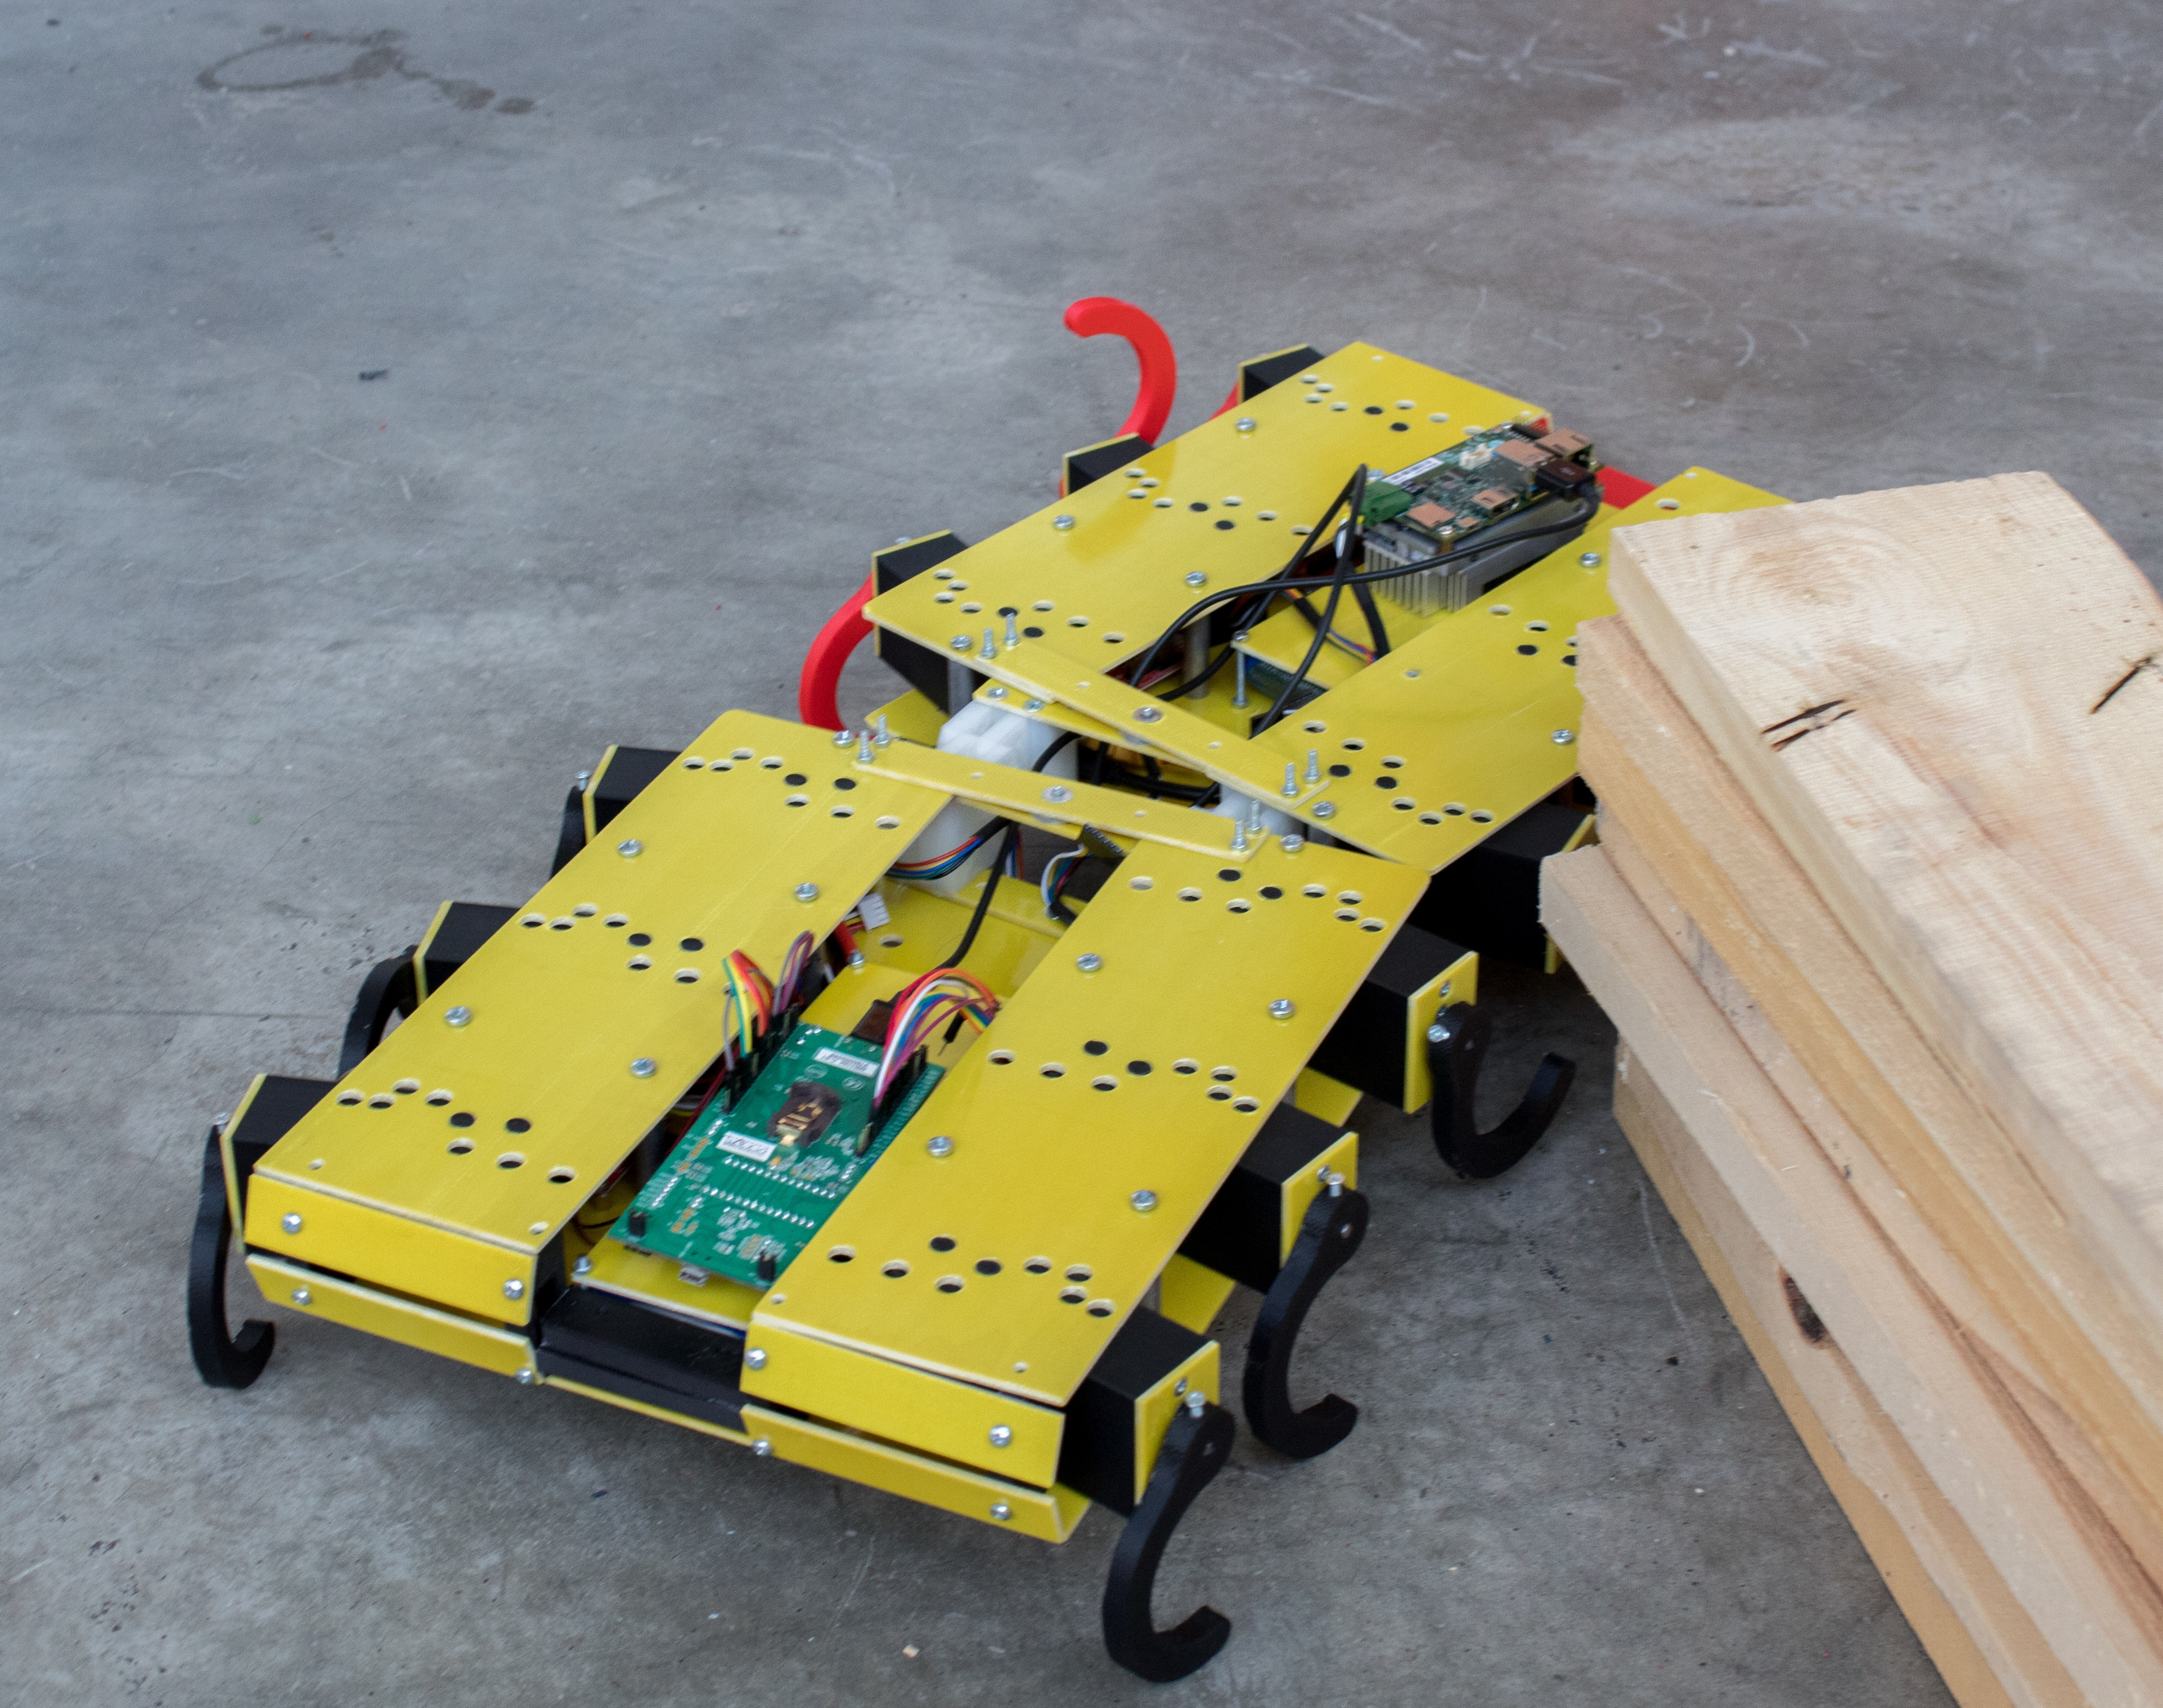
\includegraphics[width=0.49\linewidth]{strirus_2.jpg}}
        \hfill
        \subcaptionbox{Третья итерация, улучшенная\label{fig:strirus_3}}{%
        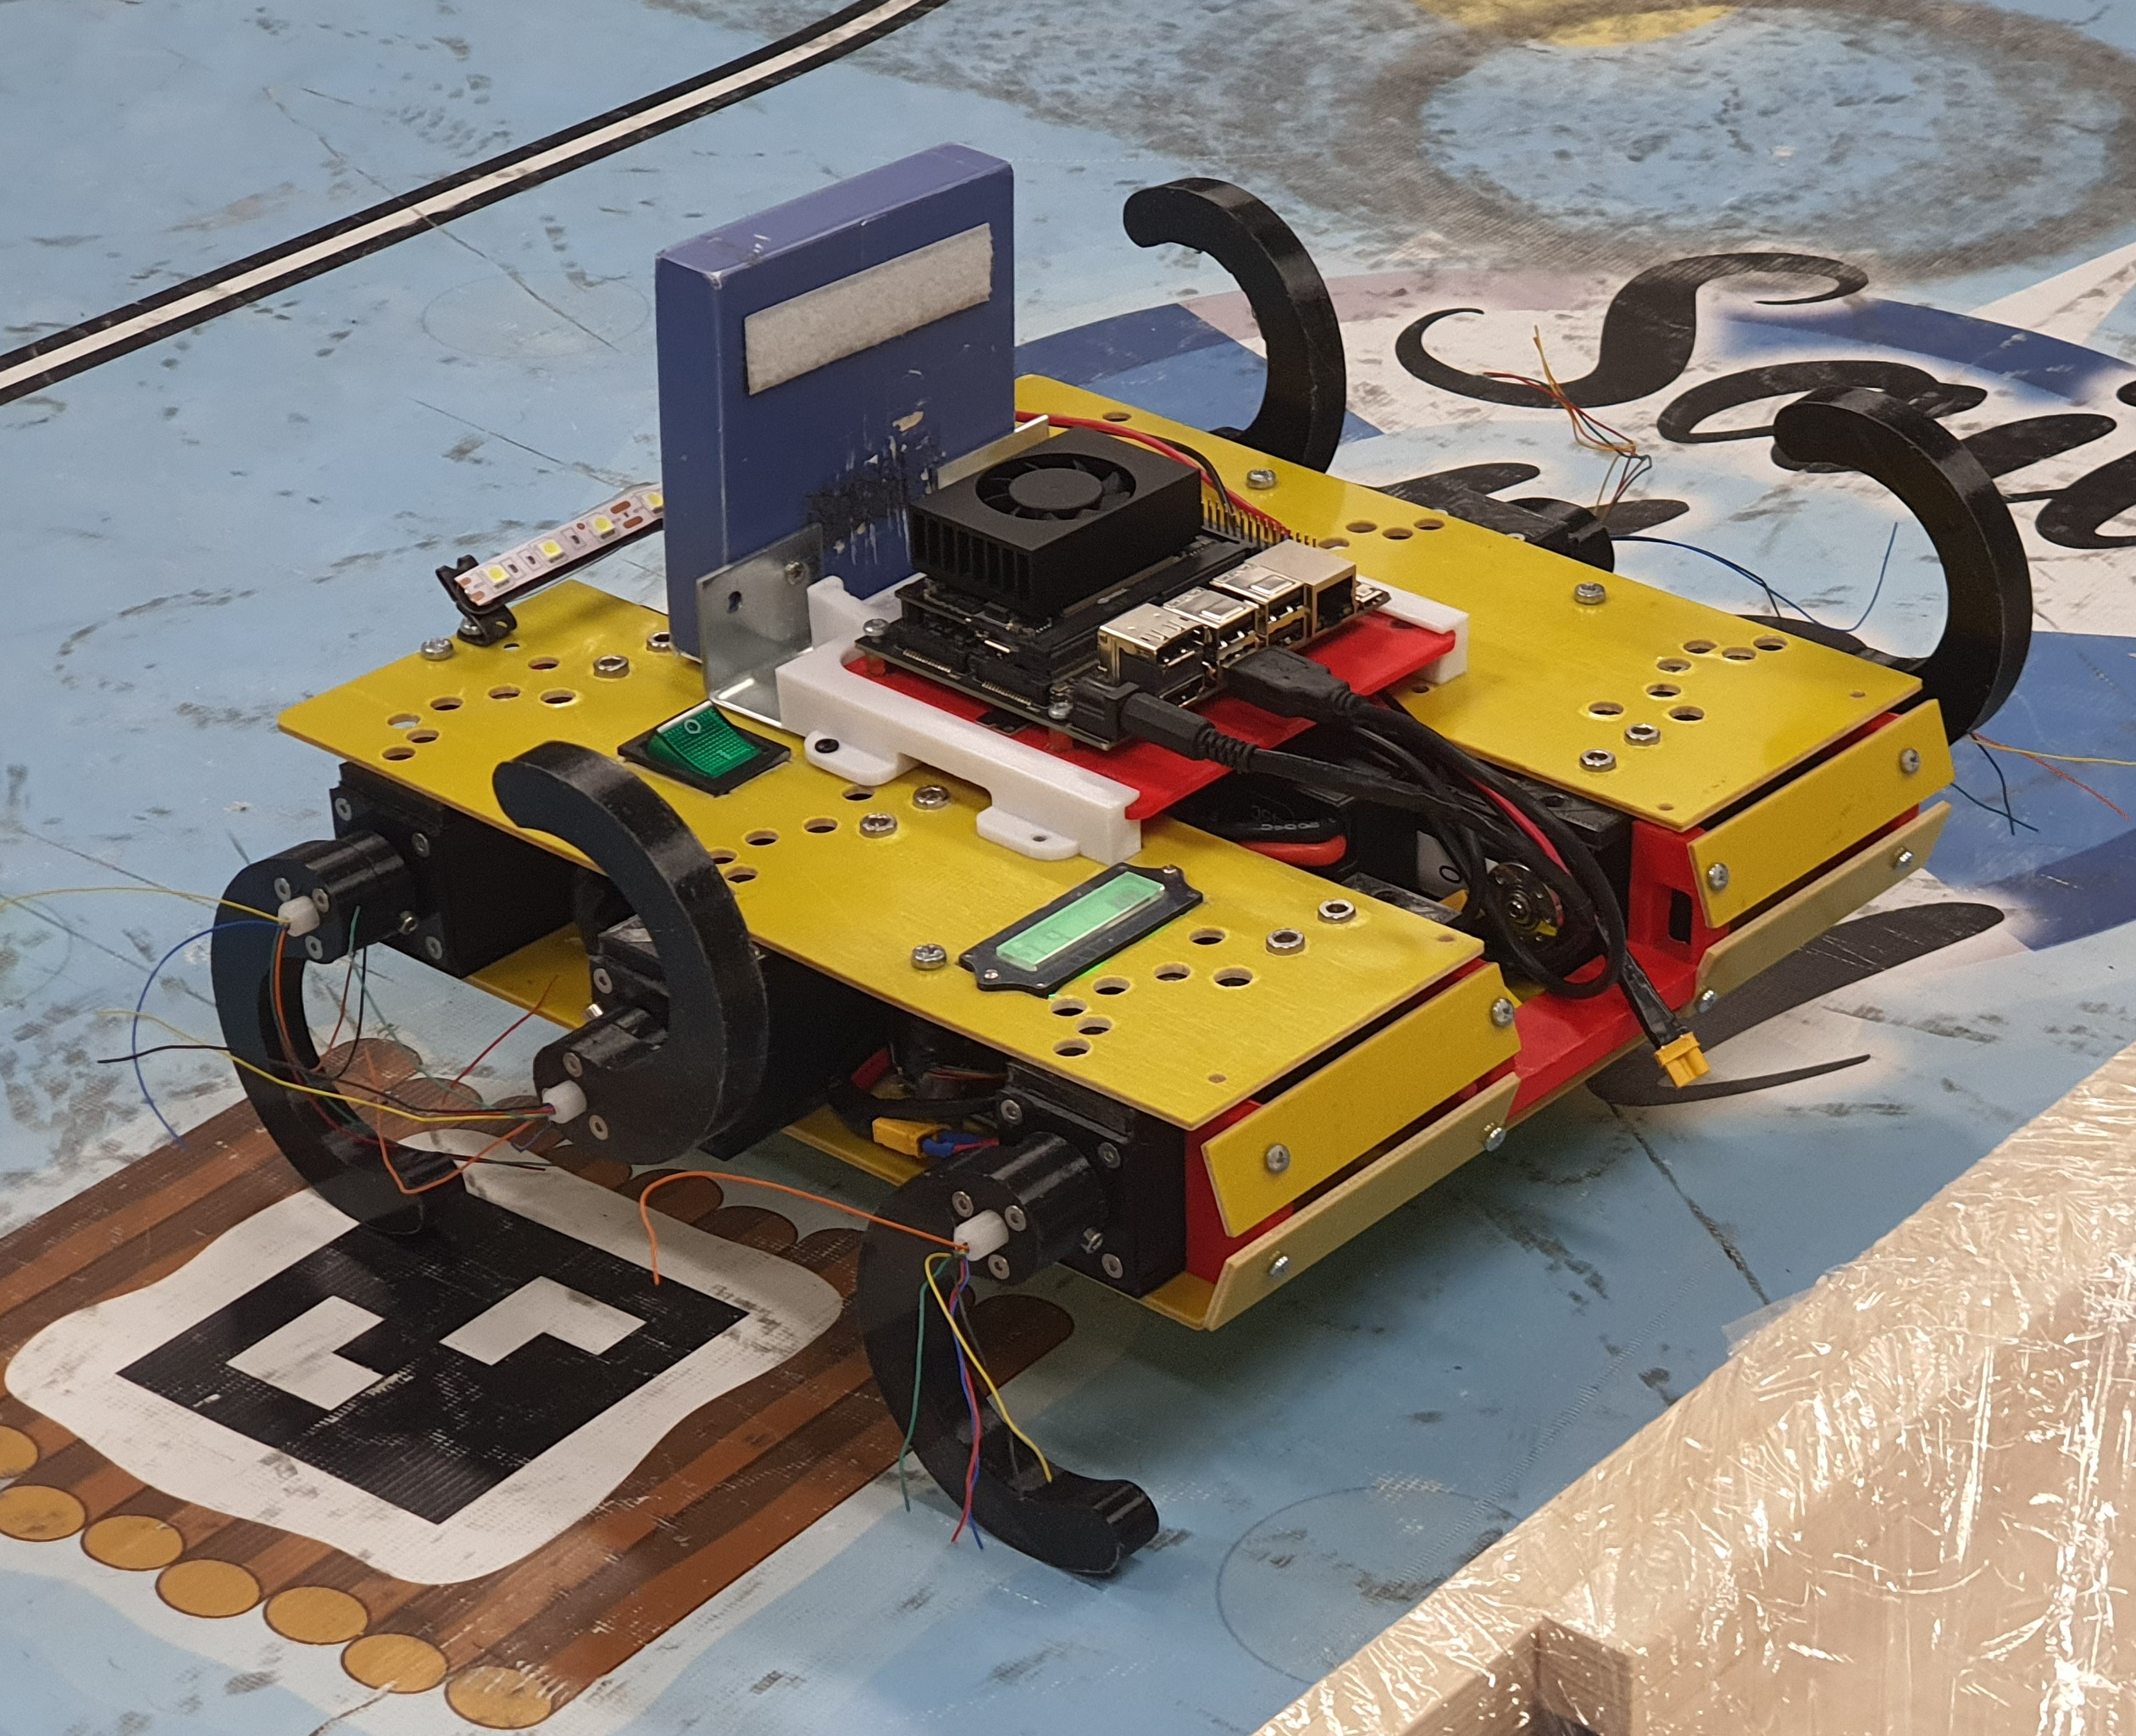
\includegraphics[width=0.49\linewidth]{strirus_3.JPG}}
        \hfill

        \subcaptionbox{Четвертая итерация\label{fig:strirus_4}}{%
        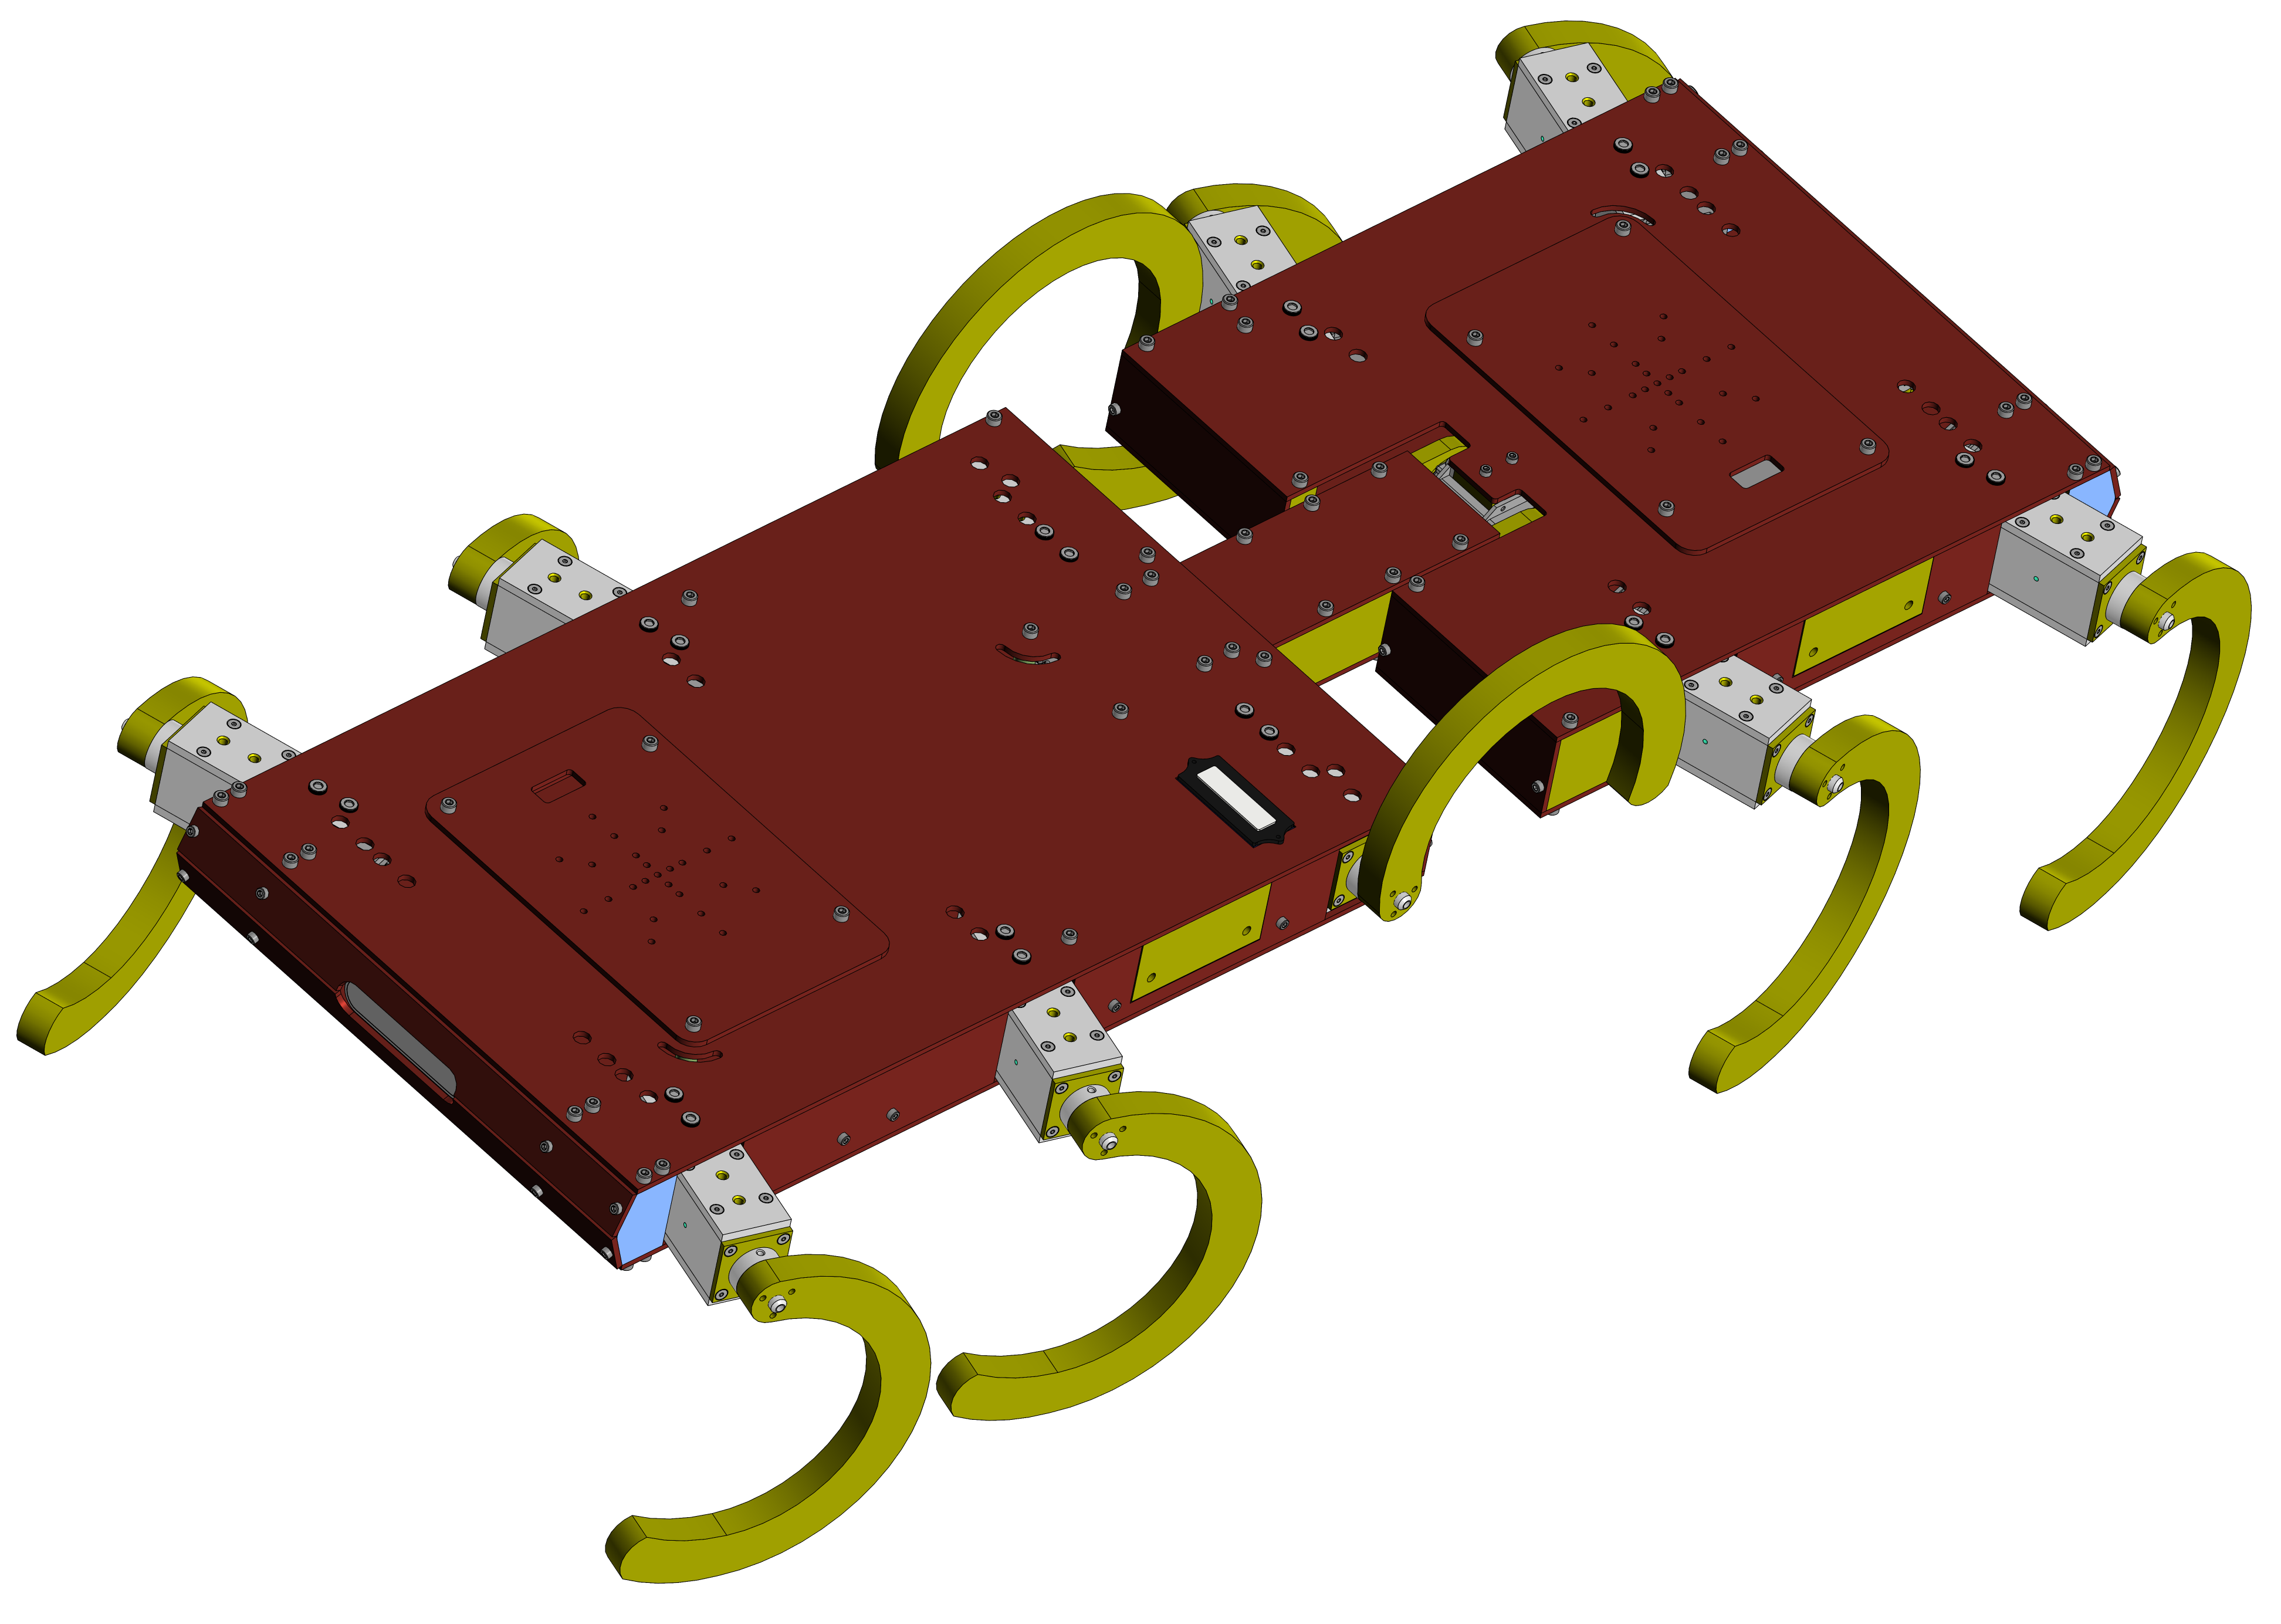
\includegraphics[width=0.9\linewidth]{strirus_4.png}}
    }
    % \legend{Подрисуночный текст, описывающий обозначения, например. Согласно
    %     ГОСТ 2.105, пункт 4.3.1, располагается перед наименованием рисунка.}
    \caption{Итерации робота СтриРуса}\label{fig:striruses}
  \end{figure}

  \begin{table}[H]
    \caption{Сравнение итераций робота}
    \label{tabular:robot_comparison_body}
    % \begin{center}
    \small
    \begin{tabular}{p{2cm}|p{2cm}|p{2cm}|p{2cm}|p{2cm}|p{2cm}}
    \toprule
    \toprule
    % \rowcolor{Gray}
     Итерация & 1 \pic{fig:strirus_0}  & 2 \pic{fig:strirus_1} &  3 \pic{fig:strirus_2} & 3+ \pic{fig:strirus_3} & 4 \pic{fig:strirus_4} \\
     \hline
     Кол-во ног & 54 & 12 & 12 & 6 & 10 \\ 
    %   \rowcolor{lightgray}
     \makecell[l]{Кол-во \\ сегментов} & 1 & 2 & 2 & 1 & 2 \\
     \makecell[l]{Тип \\ соединения} & --- & Тангаж & \makecell[l]{Тангаж,\\ рыскание} & --- & Тангаж \\
    %  \rowcolor{lightgray}
     Отн. угол телом -- нога, градусы & 0 & 0--45 & 0, 15, 30, 45 & 0 & 0, 15 \\
     \makecell[l]{Высота \\ ноги, мм} & 54 & 60 & 60 & 90 & 170 \\
     \hline
     Особенности & Волноход & Механизм, который позволяет непрерывно изменять отн. угол & Двухстепенной узел, соединяющий сегменты & Большие ноги & Гигантские ноги  \\
    %  \rowcolor{lightgray}
    \hline
     Недостатки & Невозможно установить сенсоры на ноги. Много подвижных частей & Слишком сложный механизм, изменяющий отн. угол & Мал. ноги. Избыточная вторая степень свободы в соединительном узле & 1 сегмент. Маленькие ноги & --- \\
    \bottomrule
    \bottomrule
    \end{tabular}
    % \end{center}
    \end{table}

Как итог, был разработан 10 ногий двух сегментный робот СтриРус. 10 ног было выбрано на основе результатов, полученных во время решения мультикритериальной задачи оптимизации с помощью генетического алгоритма.

Результируя вышесказанное, получив Парето решение параметрической задачи оптимизации на основе критериев проходимости,  детализации и пройденного пути было выбрано решение с 10ью ногами робота. Оптимальным углом между ногами робота при движении по плоскости оказался 120 градусов. А идея по всенаправленному движению шагающего робота без смены ориентации, основанная на концепте всенаправленного колеса нашла свое подтверждение.



